% RECOVERED COMPILE-READY READING COPY 20260708
% Generated from partial Codex-log recovery. Not the original final EA source.
\documentclass[11pt]{article}
\usepackage[a4paper,top=2.4cm,bottom=2.5cm,left=2.0cm,right=2.0cm]{geometry}
\usepackage{amsmath,amssymb,amsfonts}
\usepackage{fontspec}
\setmainfont{TeX Gyre Termes}
\usepackage{booktabs}
\usepackage{graphicx}
\graphicspath{{../}}
\usepackage[section]{placeins}
\usepackage{xcolor}
\usepackage{tikz}
\usetikzlibrary{arrows.meta,positioning}
\usepackage{caption}
\captionsetup{font=small,labelfont=bf}
\usepackage{titlesec}
\titleformat{\section}{\normalfont\large\bfseries}{\thesection}{0.6em}{}
\titleformat{\subsection}{\normalfont\normalsize\bfseries}{\thesubsection}{0.5em}{}
\titleformat{\subsubsection}{\normalfont\normalsize\bfseries}{\thesubsubsection}{0.5em}{}
\usepackage{hyperref}
\hypersetup{hidelinks}
\setlength{\emergencystretch}{3em}
\newcommand{\keV}{\ensuremath{\,\mathrm{keV}}}
\newcommand{\MeV}{\ensuremath{\,\mathrm{MeV}}}
\newcommand{\cms}{\ensuremath{\,\mathrm{cm^{-2}\,s^{-1}}}}
\newcommand{\phcms}{\ensuremath{\,\mathrm{ph\,cm^{-2}\,s^{-1}}}}
\newcommand{\cps}{\ensuremath{\,\mathrm{s^{-1}}}}
\newcommand{\wii}{W_{511}}
\newcommand{\aeff}{A_{\mathrm{eff}}}
\newcommand{\fzero}{F_{0}}
\newcommand{\fthree}{F_{3\sigma}}
\newcommand{\added}[1]{{\color{red}#1}}
\newcommand{\rewritten}[1]{{\color{green!45!black}#1}}
\newenvironment{addedblock}{\begingroup\color{red}}{\endgroup}
\newenvironment{rewrittenblock}{\begingroup\color{green!45!black}}{\endgroup}
\raggedbottom

\begin{document}
\begin{center}
{\LARGE\bfseries Detector-coupled Monte Carlo estimate of background and unresolved-line sensitivity for a balloon-borne 511 keV Laue-lens TES telescope\par}
\vspace{1em}
{\large Authors omitted for review\par}
\end{center}
\begin{abstract}
The Galactic 511 keV annihilation signal is dominated by diffuse bulge and disk emission, while compact or point-like contributions remain poorly constrained. We present a detector-coupled Monte Carlo estimate for a balloon-borne pointed telescope combining a 10 m Ge(111) Laue lens with a transition-edge sensor microcalorimeter focal plane. The signal chain transports focused 511 keV photons through the Be aperture into the detector/cryostat mass model. The background chain transports prompt atmospheric particles and photons and production-position-sampled delayed activation decays through the same model. Prompt, delayed, and signal streams are analyzed with a common $510.58$--$511.42\keV$ window, CsI anticoincidence veto, and topology/field-of-view consistency selection. For a reference point-source flux of $10^{-4}\phcms$, the selected day-15 signal and background rates are $1.18\times10^{-3}\cps$ and $4.81\times10^{-2}\cps$, respectively; prompt atmospheric events account for 91.7\% of the selected background. Folding these rates through the adopted synthetic 20 d trajectory gives $Z_{20\mathrm{d}}=7.04$ and a corresponding $3\sigma$ flux threshold of $4.26\times10^{-5}\phcms$. The result is a selected-rate flight-sensitivity estimate for a spectrally unresolved compact 511 keV source under the reference geometry and response model. Prompt atmospheric events dominate the selected background, while the delayed component is smaller but materially structured, identifying shielding, side-entry collimation, local materials, and activation validation as the main next engineering and analysis targets.
\end{abstract}
\noindent\textbf{Keywords}\hspace{0.7em}Gamma-ray instrumentation, 511 keV annihilation line, transition-edge sensors, Laue lens, balloon-borne telescope, activation background
\vspace{1em}


In this work we develop an end-to-end detector-coupled Monte Carlo chain for this concept and use it to estimate the in-flight background and point-source performance at balloon altitude and to provide directional guidance for design optimization. The chain takes the EXPACS/PARMA atmospheric cosmic-ray field as input and, at balloon altitude, transports the prompt particles while tracking their activation products, yielding both the prompt atmospheric background and the delayed activation background that builds up over the flight; the focused 511 keV reference signal is provided by a 10 m Ge(111) Laue-optics model. The signal and both backgrounds are injected into the same representative balloon-borne TES focal-plane mass model (a dilution-refrigerator cold end, passive shielding, and an active anticoincidence shield), processed with a common narrow energy window, anticoincidence veto, and topology/field-of-view selection, and folded along a reference flight trajectory to give the selected signal rate, the background composition, and the counting significance. The selected background is dominated by the prompt atmospheric component, so the shield geometry, side-entry collimation, and shield material are the most direct directions for design optimization; delayed activation enters the same evaluation as a secondary component, whereas upstream optics-hardware background remains outside the primary detector-background budget. This work thereby estimates the in-flight background and detection performance of the balloon platform and indicates directions for design optimization.

\subsection{Science and instrument requirements}
\label{sec:requirements}

The simulated instrument is aimed at 511 keV point-source or unresolved-central-excess components from the Galactic-center region that have not been detected by previous instruments. Existing INTEGRAL/SPI measurements have established a 511 keV sky dominated by diffuse bulge and disk emission and limit point-like 511 keV sources superposed on that diffuse emission to fluxes of order $10^{-4}\phcms$ \cite{Siegert2016AA,Yoneda2025}; an independent INTEGRAL/IBIS compact-source search also found no Galactic 511 keV point sources and gives an upper limit of about $1.6\times10^{-4}\phcms$ for a $\sim10$ Ms Galactic-center exposure \cite{DeCesare2011}. For a representative 511 keV atmospheric transmission of $T\simeq0.739$ at balloon altitude, this limit corresponds to an above-payload photon-flux scale of about $1.2\times10^{-4}\phcms$. The simulation therefore adopts $\fzero=10^{-4}\phcms$ as the reference point-source photon-flux scale. Compared with the wide-field spectroscopic and coded-mask searches performed by INTEGRAL, the modeled payload adds Laue focusing to improve the point-source response and uses a high-energy-resolution, multilayer thick-absorber TES microcalorimeter array as the focal-plane detector to sharpen the 511 keV line measurement \cite{Shirazi2023,Caputo2017}.

This work first considers a balloon payload as an early test platform, with the expectation that the approach can later be extended to a satellite observing platform.

This goal imposes four requirements on the instrument and the simulation: first, the telescope must concentrate 511 keV photons onto a small focal plane, so that a larger solid angle can be covered without sacrificing collecting area. Second, the focal-plane detector must provide sub-keV energy response sufficient to resolve detailed line structure. Third, the detector and shield model must suppress atmospheric, activation, and side-entry backgrounds. Fourth, the simulation chain must treat prompt background, delayed activation, focused signal, vetoes, event topology, and mission-time variation consistently, so that signal and background are evaluated under the same detector selection.

The remainder of this paper is organized as follows. Section~\ref{sec:geometry} describes the detector and cryostat mass model; Section~\ref{sec:framework} the simulation framework---the workflow, optics coupling, background sources, event selection, and mission-time fold; Section~\ref{sec:results} the selected-rate and sensitivity results together with the normalization, convergence, and boundary checks; and Section~\ref{sec:discussion} the discussion and conclusions.

\section{Detector and cryostat mass model}
\label{sec:geometry}

The detector mass model is an engineering Geant4/MEGAlib proxy mass model that contains a balloon-borne multilayer TES array mounted at the cold end of a compact dilution refrigerator (DR) \cite{Shirazi2023,Gottardi2021TESReview}. The detector model also contains typical DR cryostat structures, active shielding, passive shielding, magnetic shielding, side-entry windows, collimation structures, copper thermal structures, and other cryogenic service-mass proxies. Figure~\ref{fig:mass_model} shows two-dimensional views of the mass model used in this paper.

The TES detector concept uses an absorber-coupled AlMn film structure developed in our laboratory; the advantages of AlMn alloy include transition-temperature tunability through composition and annealing, suitability for array fabrication, and relatively low magnetic-field sensitivity \cite{Xie2026AlMn,Vavagiakis2017AlMnMagnetic}. In the present concept, the TES thermometer film is an AlMn film of order $200\,\mathrm{nm}$ thickness, whereas the $\gamma$-ray absorber is a millimetre-scale metal body. The absorber uses $1.5\times1.5\times3.0\,\mathrm{mm^3}$ Ta pixels; the high atomic number of Ta increases the interaction probability for 511 keV photons, and a $3.0\,\mathrm{mm}$ thickness corresponds to about a $49\%$ single-layer detection efficiency at 511 keV, so the six-layer array can provide near-unity detection efficiency. In the current geometry, the center-to-center spacing between adjacent Ta array layers is $12\,\mathrm{mm}$; this spacing is designed with the efficiency of the subsequent Compton-based kinematic-track veto mechanism in mind. The choice of Ta also considers its low-temperature low-specific-heat properties as a superconductor (this paper uses an order-of-magnitude estimate of $10^{-2}\,\mathrm{J\,K^{-1}\,m^{-3}}$) and a relatively high photoelectric-to-Compton interaction ratio; based on NIST XCOM cross sections near 511 keV, this ratio is about 0.731 \cite{NISTXCOM}. Based on laboratory experience and by substituting the current Ta absorber heat capacity of $67.5\,\mathrm{pJ/K}$, the simulation adopts $\Delta E_{\mathrm{FWHM}}\simeq420\,\mathrm{eV}$ at 511 keV as the current simulated energy resolution.

Because the TES film and Ta absorber differ greatly in size and mass, and because the TES film itself does not contribute significant 511 keV interactions, the transport geometry uses the Ta absorber to represent the main sensitive volume of a TES pixel. The explicit sensitive volume has six layers, 376 Ta absorber pixels per layer, and 2256 pixels in total, with 1.5 mm length and width and 3 mm thickness. A Si substrate proxy is placed below each Ta pixel, using Si to represent the SiO2-SiNx-Si substrate because this simulation does not model detailed thermal conduction. TES-film, wiring, and readout details are not built layer by layer as explicit interaction volumes; instead, they enter the model through the assumed energy response and service-mass proxies. In the current manuscript, the 511 keV line window is W511 = 511 keV $\pm$ 420 eV, i.e. 510.58--511.42 keV.

The TES array is mounted on the required copper support and thermal-link structures. Copper provides the decisive thermal-conduction path; a copper thermal finger exits through the bottom hole of the sample box and connects to the 50 mK cold plate. The near-field TES sample box serves as both magnetic shielding and local passive shielding. The current mainline geometry consists of a 2 mm Nb inner layer and a 2 mm MuMetal outer layer, with MuMetal represented in the material table as Ni:Fe = 4:1. The sample-box entrance window is covered by a thin Al window; the rear end cap retains the hole for the cold finger. A W--Nb double-layer sample box is treated as a comparison passive-shielding + magnetic-shielding material design; the X-ray window is opened on the side of the cryostat, with a 300 $\mu$m thick Al window embedded in the thermal-shield shell inside each cryostat layer, a 25 $\mu$m thick Be window placed in the vacuum shell, and an $x$-thick W collimator placed outside the Be window, with the collimator opening strictly aligned to the TES pixels. The side window is strictly defined through Boolean operations. The mass model also introduces scintillator active shielding, wrapped around the outer side wall, bottom, and top of the cryostat. Segmented CsI active shielding is used, with a radial side-shield thickness of 4 cm; the bottom and top shields are included in the geometry as axial end volumes. CsI volumes enter the simulation as transport and activation materials, and their deposited energies are read in post-processing to apply the active veto; the counting threshold is 50 keV. BGO active shielding is treated as a material-comparison case; the BGO threshold is 70 keV. Considering the physical layout of the DR and the side-entry optical path, the cryostat instrument frame is rotated as a whole by 45 degrees, so that the local side window is tilted $45^\circ$ upward in the zenith-frame source coordinates.

\begin{figure}[t]
\centering
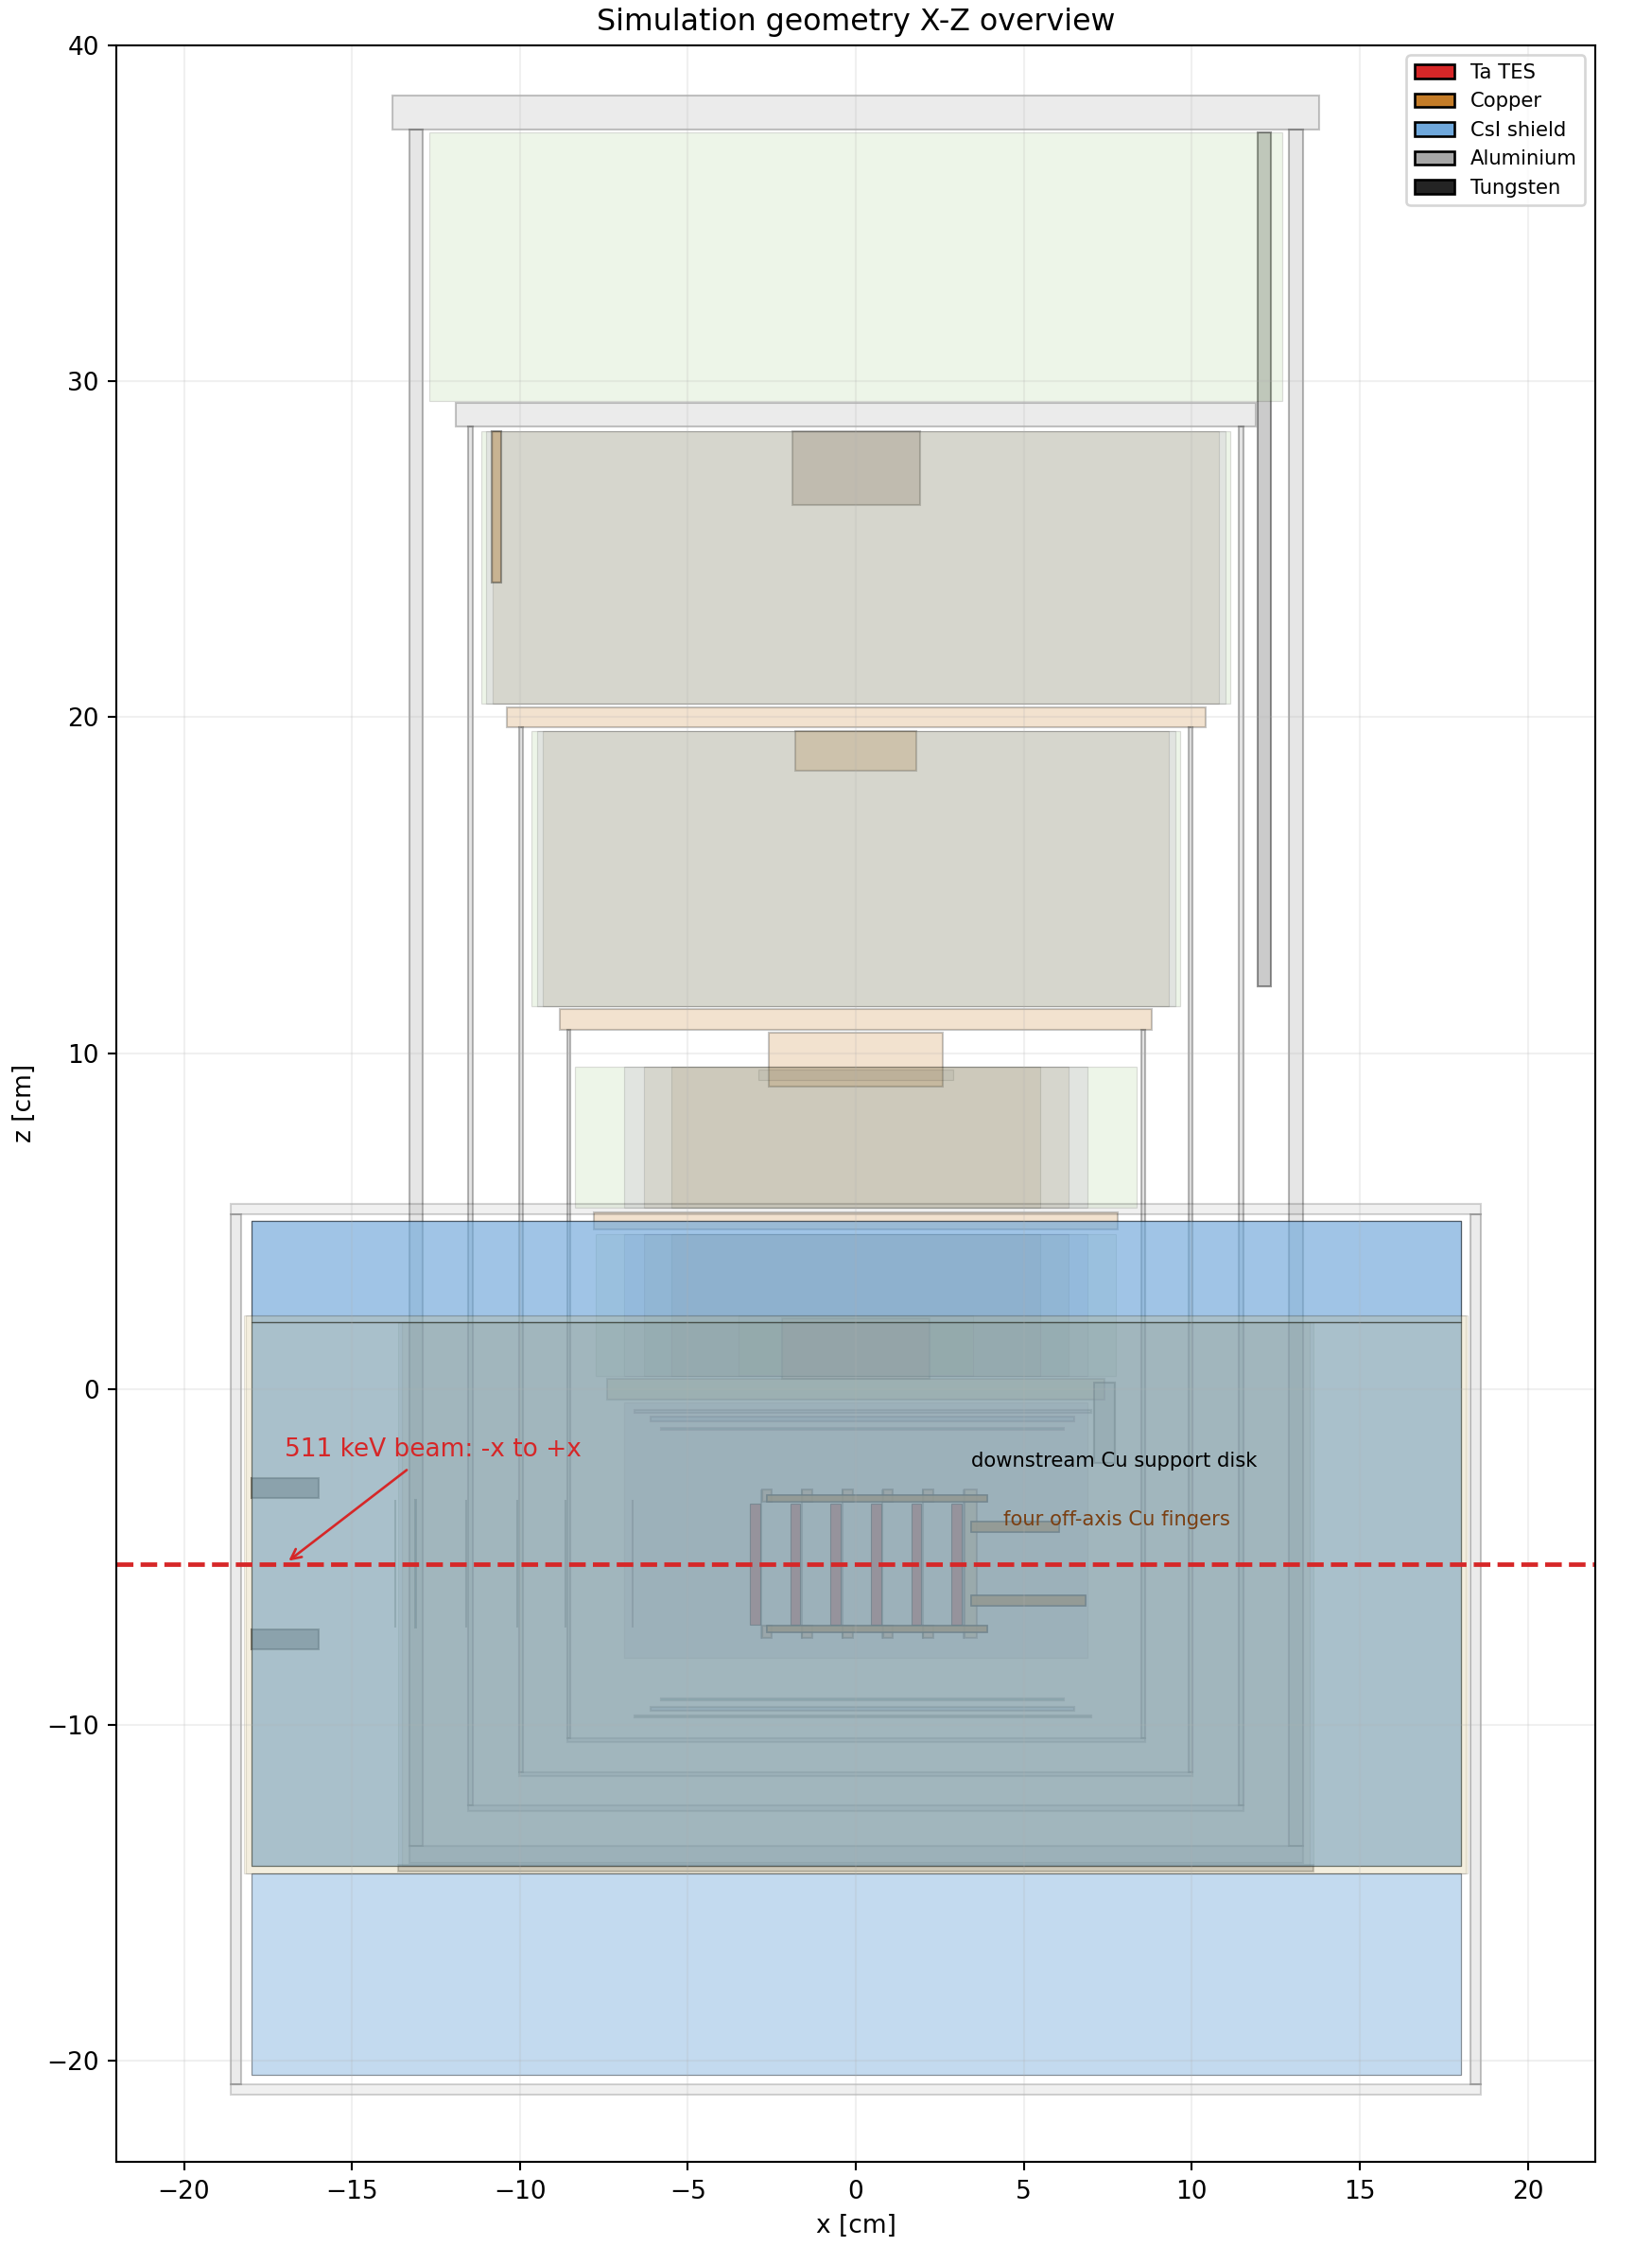
\includegraphics[width=0.62\linewidth]{paper_source_figure_table/fig_mass_model_xz_overview.png}
\caption{Two-dimensional overview of the detector/cryostat proxy mass model, showing the X--Z view of the DR tower, detector bay, active shield, and 511 keV side-entry beam path.}
\label{fig:mass_model}
\end{figure}

\FloatBarrier

\section{Simulation framework}
\label{sec:framework}

Detector-coupled Monte Carlo transport through detailed mass models is a mature method for predicting the response and background of gamma-ray spectrometers \cite{Sturner2003}. This section describes the full end-to-end simulation chain from source generation to flight-performance assessment. The focusing optics and detector system start from independent mass models: the optics-branch mass model takes the target point source and records focused photons reaching the focal-plane plane as the focused-source input to the detector branch; the detector branch then directly transports, in the detector/cryostat mass model of Section~\ref{sec:geometry}, prompt atmospheric particles, delayed decays generated from activation products according to recorded production positions, and the focused sources described above. The focused source, prompt source, and delayed source are simulated stepwise and normalized onto one time axis through Poisson-statistics-based time-axis sampling and renormalization, then the background is further suppressed by scintillator-based active veto and Compton-kinematics-based veto. The chain subsequently enters detailed background-analysis statistics, analysis of signal and background intensity variation caused by mission flight-time trajectory changes, and the overall flight-performance assessment and design-optimization recommendations. Because the focused signal and the two background streams all pass through the same response and veto definitions before any background decomposition or sensitivity statement, the subsequent results rest on a consistent event selection.

Figure~\ref{fig:workflow} expands this chain by computational layer: geometry definition, prompt and activation-accumulation transport, delayed-source construction, focused-optics transport, detector-coupled signal replay, veto mechanisms, detailed background analysis, time/flight-trajectory variation, and flight-performance assessment with design-optimization recommendations. The following subsections describe each layer's inputs, operations, and outputs.

The above simulation is for a specific balloon-flight moment, longitude and latitude, and altitude. Although for an observation time such as one hour equivalent to several Monte Carlo events, this position can be regarded as constant. However, for a long-time flight on the scale of days, the altitude, longitude, and latitude obviously change significantly. This causes changes in the magnetic-rigidity cutoff for instantaneous cosmic rays and changes in the atmospheric transmission for the signal, and the activation background itself also changes with the incident cosmic-ray flux and different stages of the decay chain. This reminds us that the background-signal at a reference moment should not be linearly extrapolated in time to evaluate the time-folded flight performance over the whole working time. Therefore, we introduce a reasonable analytical flight-trajectory--time curve to evaluate the performance over the whole working cycle, and simulate multiple points on the curve to verify the rationality of the curve.

\begin{figure}[t]
\centering
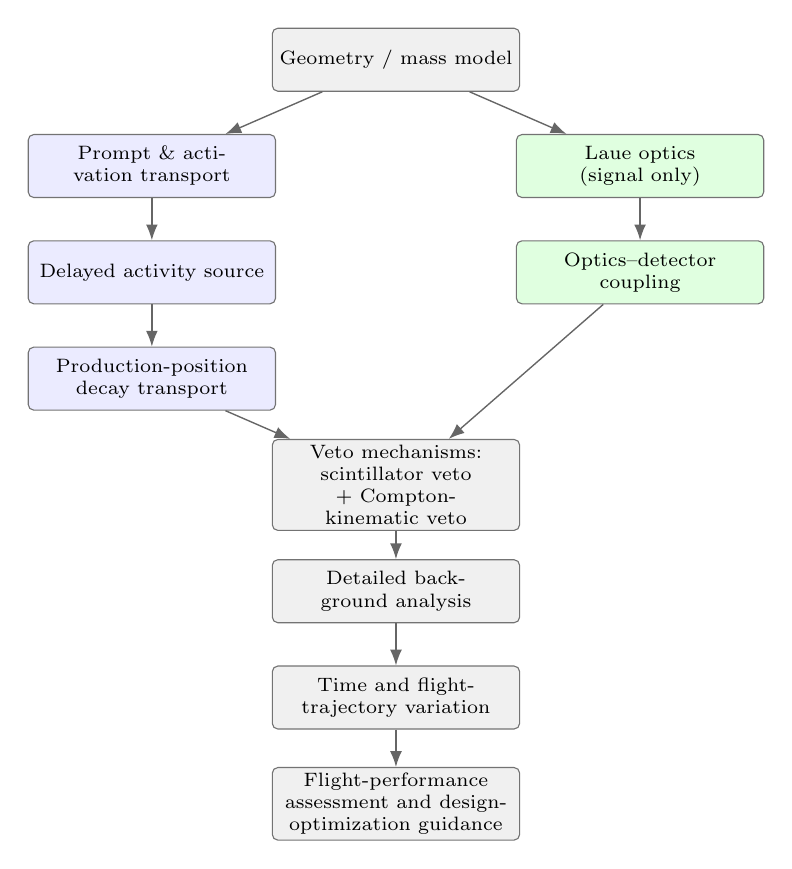
\begin{tikzpicture}[
  box/.style={rectangle, rounded corners=2pt, draw=black!55, line width=0.4pt,
              align=center, font=\scriptsize, text width=30mm, minimum height=8mm, inner sep=2pt},
  bg/.style={box, fill=blue!8},
  sig/.style={box, fill=green!12},
  shr/.style={box, fill=black!6},
  flow/.style={-{Latex[length=2mm]}, draw=black!60, line width=0.5pt}
]
\node[shr] (geo)    at (0,0)        {Geometry / mass model};
\node[bg]  (prompt) at (-3.1,-1.35) {Prompt \& activation transport};
\node[bg]  (delay)  at (-3.1,-2.7)  {Delayed activity source};
\node[bg]  (decay)  at (-3.1,-4.05) {Production-position decay transport};
\node[sig] (optics) at (3.1,-1.35)  {Laue optics (signal only)};
\node[sig] (couple) at (3.1,-2.7)   {Optics--detector coupling};
\node[shr] (sel)    at (0,-5.4)     {Veto mechanisms: scintillator veto $+$ Compton-kinematic veto};
\node[shr] (detail) at (0,-6.75)    {Detailed background analysis};
\node[shr] (fold)   at (0,-8.1)     {Time and flight-trajectory variation};
\node[shr] (out)    at (0,-9.45)    {Flight-performance assessment and design-optimization guidance};
\draw[flow] (geo) -- (prompt);
\draw[flow] (geo) -- (optics);
\draw[flow] (prompt) -- (delay);
\draw[flow] (delay) -- (decay);
\draw[flow] (optics) -- (couple);
\draw[flow] (decay) -- (sel);
\draw[flow] (couple) -- (sel);
\draw[flow] (sel) -- (detail);
\draw[flow] (detail) -- (fold);
\draw[flow] (fold) -- (out);
\end{tikzpicture}
\caption{Simulation chain used in this work. Blue nodes are the prompt and
delayed background streams, green nodes the focused-signal optics, and grey
nodes the shared geometry, veto mechanisms, detailed background analysis,
time/trajectory variation, and final flight-performance assessment. The focused
signal and all background streams are evaluated under the same detector response
and veto definitions before background decomposition, mission-time variation,
and design-optimization judgments are made.}
\label{fig:workflow}
\end{figure}

\FloatBarrier

\subsection{Laue optics and detector-coupled signal replay}
\label{sec:optics}

This simulation adopts a laue-lens system based on mosaic Ge(111) crystals \cite{Barriere2009Laue,Barriere2011LauePrototype}. Through optical design, it realizes a 10 m focal length, a 511\keV{} single-ring reference response, and an effective area of $20.1\,\mathrm{cm^2}$ at 511\keV; the effective area is calculated as
\begin{equation}
  A_{\mathrm{eff}}(E)=A_{\mathrm{inc}}\frac{N_{\mathrm{fp}}(E)}{N_{\mathrm{inc}}(E)}
  \label{eq:laue_aeff}
\end{equation}
where $A_{\mathrm{inc}}$ is the Monte Carlo incident sampling area, $N_{\mathrm{inc}}(E)$ is the number of incident photons, and $N_{\mathrm{fp}}(E)$ is the number of photons satisfying the focusing/focal-plane interception condition.
The mosaic system is adopted to make the Monte Carlo calculation convenient while satisfying the expected focusing performance; other candidate schemes are also possible for actual engineering adaptation.

In this simulation, the laue optical branch gives the focusing-performance simulation and transports the focused signal through the Ge crystal mass.

For this purpose, the diffraction probability of photons by the crystal is no longer superposed onto photons as an efficiency parameter, but is defined as a discrete process at the Geant4 application layer \cite{Agostinelli2003,Allison2016}. The process takes the diffraction probability $R(|\Delta\theta|)$ according to the angular deviation of the current photon relative to the crystal plane, and converts it into a finite equivalent diffraction mean free path $\lambda_{\mathrm{diff}}$, so that the accumulated diffraction probability when the photon crosses a crystal path $\ell$ reproduces this value: $1-\exp(-\ell/\lambda_{\mathrm{diff}})=R(|\Delta\theta|)$, namely $\lambda_{\mathrm{diff}}=-\,\ell/\ln[1-R(|\Delta\theta|)]$; to avoid double counting with standard photoelectric absorption, $R$ is first normalized by the unabsorbed fraction ($R/(1-A)$) and then converted into a mean free path. After this mean free path is returned to Geant4, the diffraction process and the standard electromagnetic processes (photoelectric absorption and Compton scattering) each sample interaction lengths in the same competition framework, and the shortest one decides which process occurs first, rather than forcibly intercepting photons at the crystal boundary. Photons not selected to undergo diffraction still continue transport according to the standard electromagnetic physics, and may be absorbed, scattered, or directly transmitted.

The diffraction probability is preferentially given by interpolation in an external XOP/CRYSTAL rocking-curve map as a function of angular deviation: this curve is calculated offline once in the preprocessing stage by the CRYSTAL/diff\_pat module of the XOP toolkit (called through xoppylib, with DABAX crystallographic data as input) \cite{SanchezDelRio2011XOP}, and gives the Ge(111) reflectivity/transmissivity/absorption curves as a function of angular deviation; during transport, the angular deviation is calculated in real time for every step inside the crystal, and the current diffraction probability is obtained by interpolation on that curve, namely ``offline library tabulation, probability used by angle during transport''. The mosaic orientation is implemented by applying a Gaussian angular perturbation to the ideal Bragg-plane normal, with the perturbation width given by the 30 arcsec mosaic FWHM; after diffraction occurs, the outgoing direction is mirror-reflected according to the perturbed plane normal, and the photon energy is unchanged. This split in which the ``process class only handles the transport interface, and the independent model class handles probability and direction decisions'' follows the idea of existing crystal Bragg-reflection extensions in Geant4 \cite{Guan2023BraggReflection,Reiazi2025G4BraggReflection}, and extends it to the energy band needed here.

Here the reference signal is a monochromatic 511\keV{} point source whose flux scale is set by the INTEGRAL/SPI upper limit on a compact 511\keV{} source superposed on the Galactic-centre diffuse emission ($\fzero=10^{-4}\phcms$ above the atmosphere, Section~\ref{sec:requirements}) \cite{Siegert2016AA,DeCesare2011}, rather than by any single observed object. It is constructed as a MEGAlib far-field source \cite{Zoglauer2006}, with the detailed construction given in Section~\ref{subsec:pointsource}. The signal is transported through the optics branch and injected into the detector mass model as a parallel-beam source; prompt cosmic-ray background and activation decays are transported directly in the detector/cryostat mass model. Optics-mass prompt and delayed background are not included in the primary detector-background budget.

\subsection{Source construction}
\label{sec:background}

After the focusing optics have been defined in Section~\ref{sec:optics}, the
optical input and the subsequent detector input require three source layers: the
prompt atmospheric particle field incident on the payload, the delayed
radioactive population accumulated in the instrument by that particle field, and
the reference signal point source. These three layers are constructed
separately, rather than running transport by directly invoking MEGAlib's buildup
function for them at the same time, in order to reduce computational cost.

\subsubsection{Prompt atmospheric source}
\label{subsec:prompt_source}

The prompt atmospheric field is derived from EXPACS/PARMA. PARMA3.0 is an
analytical model parameterized from PHITS atmospheric-shower calculations and
benchmarked against terrestrial cosmic-ray measurements, and EXPACS is its
public tabulation and software interface
\cite{Sato2015EXPACS,Sato2016PARMA4}. PHITS supplies the underlying
particle-transport physics: primary cosmic rays interact with air nuclei, the
secondary hadrons, leptons, photons, and neutrons are transported through the
atmospheric column, and the resulting fluences are parameterized by altitude,
geomagnetic cutoff, solar modulation, energy, and direction. In this work
EXPACS/PARMA provides the differential incident flux as a function of particle
species, kinetic energy, zenith angle, geographic position, altitude, cutoff
rigidity, and solar activity, and is used only to construct the external
radiation fields; detector response, vetoing, topology selection, and
mission-time counting are applied downstream. The reference source definitions
use latitude $34^\circ$, longitude $100^\circ$, altitude $38\,\mathrm{km}$,
vertical cutoff rigidity $R_c=11.6\,\mathrm{GV}$, and the 2025-08-31 solar
condition corresponding to $W=118.3$.

The prompt source includes photons, neutrons, electrons, positrons, protons,
alpha particles, and negative and positive muons. For each particle family the
EXPACS/PARMA differential spectrum is converted into a MEGAlib far-field area
source covering the full zenith range $\theta=0^\circ$--$180^\circ$ and full
azimuth range $\phi=0^\circ$--$360^\circ$. The zenith dependence is represented
by 20 differential equal-$\mu$ angular bins, where $\mu=\cos\theta$ and each
bin subtends $\Delta\Omega=0.6283185307\,\mathrm{sr}$: the first ten bins cover
down-going particles, the last ten up-going or albedo-like particles. Both
hemispheres are retained in the prompt transport and in the
activation-production transport, so upward albedo particles are not discarded
at source construction. Figure~\ref{fig:expacs_fullsphere_flux} shows the
resulting full-sphere flux field.

\begin{figure}[t]
\centering
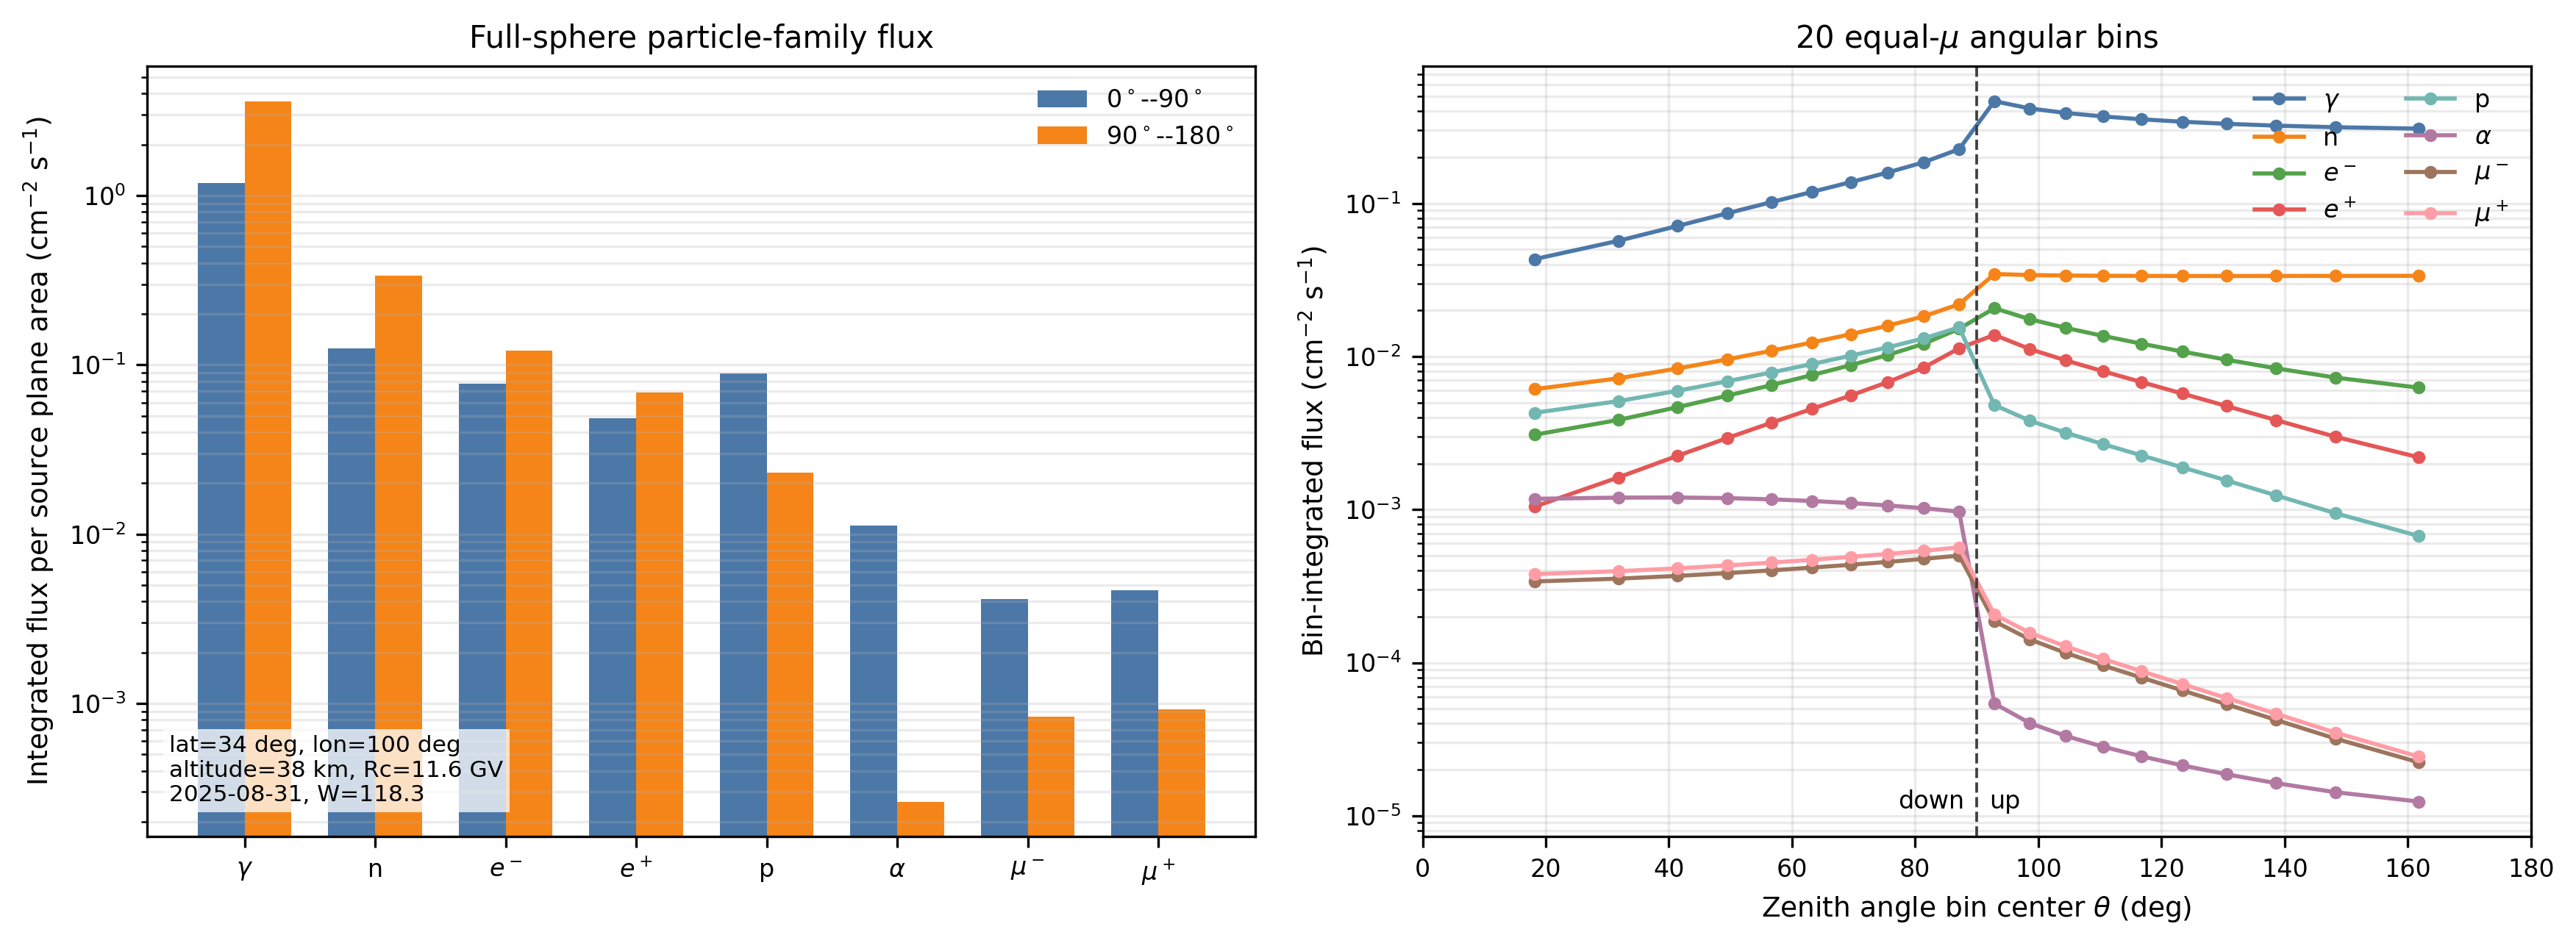
\includegraphics[width=\linewidth]{paper_source_figure_table/fig_expacs_fullsphere_flux.png}
\caption{EXPACS/PARMA full-sphere atmospheric flux field used to generate the prompt and activation-production transport inputs. Left: energy- and solid-angle-integrated fluxes for the eight transported particle families, separated into down-going and up-going hemispheres. Right: bin-integrated flux in the 20 equal-$\mu$ differential zenith bins used by the MEGAlib far-field source. The plot is generated from the source-definition inputs for latitude $34^\circ$, longitude $100^\circ$, altitude $38\,\mathrm{km}$, $R_c=11.6\,\mathrm{GV}$, and $W=118.3$.}
\label{fig:expacs_fullsphere_flux}
\end{figure}

The integrated source-plane fluxes are approximately $4.80$, $0.462$, $0.199$,
$0.117$, $0.112$, $0.0115$, $0.0050$, and $0.0056\,\mathrm{cm^{-2}\,s^{-1}}$
for $\gamma$, $n$, $e^-$, $e^+$, $p$, $\alpha$, $\mu^-$, and $\mu^+$,
respectively; the non-photon families together carry about
$0.91\,\mathrm{cm^{-2}\,s^{-1}}$, or 16\% of the total. If Monte Carlo counts
were allocated strictly in proportion to flux, the detector and activation
statistics of these minority families would be poor, so the non-photon
families are generated with replicated samples and de-weighted in the rate
normalization. All particles are then transported through the
detector/cryostat mass model with Geant4/MEGAlib
\cite{Agostinelli2003,Allison2016,Zoglauer2006}; the prompt run and the
activation-production run each generated 25,210,216 incident primaries. Each
particle species is normalized with its own transported exposure,
\begin{equation}
  r_{\mathrm{event},j}=\left(\sum_i \mathcal{T}_{ij}\right)^{-1},
\end{equation}
where $\mathcal{T}_{ij}$ is the transported exposure of subsample $i$ for
species $j$. This per-species normalization is required because the photon and
non-photon streams have different sampling and exposure structures; the
normalization check enforces $r_{\mathrm{event},j}\sum_i\mathcal{T}_{ij}=1$
for every species, so over-sampling changes the Monte Carlo variance but not
the expected physical rate.

\subsubsection{Delayed activation source}
\label{subsec:delayed_source}

For the delayed simulation, a separate activation-production stream is run by
enabling BUILDUP during the prompt-background transport. This
activation-production stream is not counted as an immediate detector background.
Instead, it records the isotope, material volume, and production position of
each radioactive product. These records are converted through the
production--decay accumulation equation into a radioactive population fixed to a
chosen reference time during the flight, with ground-state half-lives checked
against NUBASE2020 \cite{Kondev2021NUBASE}. For isotope $k$,
\begin{equation}
  A_k(t_{\mathrm{flight}}) = P_k\left[1-\exp\left(-\lambda_k t_{\mathrm{flight}}\right)\right],
  \qquad \lambda_k = \frac{\ln 2}{t_{1/2,k}},
\end{equation}
where $P_k$ is the production rate inferred from the activation-production
transport and $t_{\mathrm{flight}}=15\,\mathrm{d}$ for the reference state.
The fixed delayed total activity used by the reference delayed-source
construction is $141.83\,\mathrm{Bq}$.

The position information does not come from the aggregate isotope store alone.
The standard store records volume names and isotope counts; the
production-position construction adds a custom recording hook in the MEGAlib
stepping-action layer. Whenever a delayed isotope is stored during activation
buildup, the hook writes a production-position record at the same moment,
including the logical volume name, pre-step position $(x,y,z)$, isotope
identifier $1000Z+A$, excitation energy, time, process, and track-ancestry
information. The fixed day-15 population is then matched to these records by
volume, isotope, and excitation state, so the delayed source can use the
simulated production coordinates rather than only volume-integrated activities.
The current Mass\_model\_511 source-level inventory is dominated by CsI-shield
activation and $^{128}$I, with smaller contributions from Cu, Al, W, Mg, and
Cs isotopes. A Mass-specific appendix position-distribution figure remains to
be regenerated. It is a source-construction diagnostic, not a detector-count
map; detector response is applied only after the delayed
decays are transported through the common geometry and event selection.

Whether the production positions are worth preserving can be tested from the
same table. Delayed decays are emitted locally, so downstream attenuation,
active-shield veto probability, and event topology all depend on where the
isotope was produced, and different incident families---with their different
energy-loss, stopping, and capture histories---need not deposit their
activation in the same materials. To quantify this, the weighted production
rows are grouped by incident particle family and material category, and the
activity-normalized category distributions of two families $a$ and $b$ are
compared with the total-variation distance
\begin{equation}
  D_{\mathrm{TV}}(a,b) =
  \frac{1}{2}\sum_c \left| f_{a,c} - f_{b,c} \right| ,
\end{equation}
where $f_{a,c}$ is the fraction of delayed activity from family $a$ produced
in material category $c$. In the fixed day-15 table, neutron-induced products
carry about $133.67\,\mathrm{Bq}$, $\mu^-$-induced products $7.63\,\mathrm{Bq}$,
proton-induced products $0.434\,\mathrm{Bq}$, and $\alpha$-induced products
$0.0825\,\mathrm{Bq}$, with smaller $\mu^+$, $e^+$, and $\gamma$ terms. The
neutron-induced activity remains dominated by the CsI shield. The corresponding
Mass\_model\_511 material-category fractions have not yet been regenerated.
A volume-integrated or axisymmetric radial source could preserve the total
activity, but it would erase these incident-family, material, nuclide, and
coordinate correlations; the production-position construction keeps them in
the source before detector transport.

The delayed-decay source is therefore emitted from sampled production positions
rather than from an axisymmetric distribution. Let row $j$ in the weighted
production table have activity weight $w_j$, with total activity
$A=\sum_j w_j$. During construction, $M$ production positions are drawn with
replacement using probability $p_j=w_j/A$, and each sampled point source is
assigned the same flux $A/M$. The expected activity assigned to row $j$ is
\begin{equation}
  \mathbb{E}\!\left[N_j\frac{A}{M}\right] = M p_j \frac{A}{M} = w_j ,
\end{equation}
so the estimator preserves the total activity and is unbiased for the weighted
spatial distribution. Here $M$ is the number of equal-activity sampled point
sources; it is a sampling size, not the number of physical production rows. The
reference delayed source preserves the fixed total activity at the
source-definition level and is replayed through the same detector/cryostat
geometry as the prompt stream. The nominal calculation transports $10^6$
delayed decays; the corresponding Cosima live time is only the transport record
used to generate the decay sequence and is not used as the physical balloon
exposure time.

Table~\ref{tab:background_source_model} summarizes the source layers used in the
current detector-coupled calculation. It is placed in the source-model section
because this section defines incident particle fields and delayed radioactive
populations; detector vetoes and topology selections are applied only in the
subsequent selection section.

\begin{table}[t]
\centering
\caption{Background-source layers used by the current detector-coupled chain. The table defines source construction only; anticoincidence, topology selection, and the line window are applied later in Section~\ref{sec:selection}.}
\label{tab:background_source_model}
\begin{tabular}{p{0.22\linewidth}p{0.34\linewidth}p{0.34\linewidth}}
\hline
Layer & Physical role & Current implementation \\
\hline
Prompt atmospheric transport & Direct detector hits from atmospheric secondaries & EXPACS/PARMA full-sphere source definitions at $34^\circ$ latitude, $100^\circ$ longitude, $38\,\mathrm{km}$ altitude, $R_c=11.6\,\mathrm{GV}$, and $W=118.3$; $\gamma$, $n$, $e^\pm$, $p$, $\alpha$, and $\mu^\pm$ over 20 equal-$\mu$ differential zenith bins including both down-going and up-going hemispheres; 25,210,216 generated primaries. \\
Activation production & Radioisotope production and production-position history & Same atmospheric field transported as a BUILDUP activation-production stream, again retaining both hemispheres and all eight particle families; 25,210,216 generated primaries. \\
Fixed delayed population & Radioactive activity at the adopted day-15 state after continuous exposure & Production--decay accumulation with NUBASE-checked ground-state half-lives; total fixed activity $141.83\,\mathrm{Bq}$. \\
Production-position decay transport & Delayed decay particles emitted from sampled production positions & Equal-activity sampled point sources from the weighted production table; reference transport uses $10^6$ delayed decays per source sampling. \\
\hline
\end{tabular}
\end{table}

This production-position representation does not create one sampled point source
for every production row. It is a statistical sampling approximation whose
adequacy remains to be evaluated at the selected-rate level. Source-list checks
verify activity conservation and source serialization; selected-rate behavior
remains to be tested after detector transport and event selection.

\subsubsection{Reference point-source construction}
\label{subsec:pointsource}

The focused signal stream is defined by a monochromatic 511\keV{} reference
point source. Its flux scale is set not by any single observed object but by the
INTEGRAL/SPI upper limit on a compact 511\keV{} source superposed on the
Galactic-centre diffuse emission, $\fzero=10^{-4}\phcms$ above the atmosphere
(Section~\ref{sec:requirements}) \cite{Siegert2016AA,DeCesare2011}.

Because such a source lies at astronomical distance, it is modelled as an ideal
on-axis point: in the optics run it is a monochromatic 511\keV{} far-field beam
whose photons arrive parallel to the optical axis and are sampled uniformly over
the incident aperture $A_{\mathrm{inc}}$ of Eq.~(\ref{eq:laue_aeff}). No finite
angular size is assigned to the source itself; the angular structure that reaches
the focal plane is produced entirely by the lens---the 30 arcsec mosaic spread,
the XOP/CRYSTAL rocking curve, and the $f=10\,\mathrm{m}$ focusing geometry---so
that the replayed beam converges to within about $0.4^\circ$ of the axis and
forms a focused spot rather than a single ray. Three independent seeds of
$5\times10^{4}$ primaries each give $1.5\times10^{5}$ transported photons, of
which 37,256 are diffracted and cross the focal plane; 37,194 of these (99.8\%)
fall within the $r=1.898\,\mathrm{cm}$ Be entrance window, with focused-spot
radii $r_{90}=1.03\,\mathrm{cm}$ and $r_{99}=1.25\,\mathrm{cm}$. The
within-window crossings form the event list that is replayed through the Be
aperture into the detector/cryostat model with the recorded positions and
directions.

The normalization ties this replay to the reference flux. At the detector
entrance the focused stream carries the rate $\fzero\,\aeff(511\keV)\,T$, where
$\aeff(511\keV)=20.1\,\mathrm{cm^2}$ is the on-axis effective area and $T=0.739$
is the reference 511\keV{} atmospheric transmission at the day-15 trajectory
anchor; numerically this is $1.48\times10^{-3}\cps$ at the reference flux.
Equivalently, the generating run corresponds to an observation time
$N_{\mathrm{fp}}/[\fzero\,\aeff\,T]$, and each replayed event carries the inverse
of that exposure as its rate weight; in the intermediate cut-flow bookkeeping of
Section~\ref{sec:selection} the same sample appears as a unit replay before this
scale is applied. After the common detector response and event selection, the
surviving signal rate is $1.185\times10^{-3}\cps$, corresponding to a selected
effective area of $S_{\wii}/\fzero=11.85\,\mathrm{cm^2}$. Because the optics run
contains only source photons, the replayed stream is signal-pure; all
backgrounds enter through the streams of Section~\ref{sec:background}.

The effective area quoted above is the on-axis value, representing best-case
pointing. A point source offset from the optical axis, or residual attitude
jitter during flight, reduces and shifts the focused response through the finite
angular acceptance (field of view) of the Laue lens
\cite{Barriere2009Laue,Weidenspointner2006MAX}; this off-axis dependence is
treated as a pointing systematic on the signal effective area rather than as a
change to the on-axis reference construction. The current $45^\circ$
side-entry response is a north-sky/near-zenith reference, not a simulated
low-elevation Galactic-centre observation.

\subsection{Detector event selection and veto definitions}
\label{sec:selection}

The detector-level selection chain places the focused-signal, prompt
atmospheric, and delayed-activation streams on one common time axis and applies
two veto layers in sequence. Because both veto layers are defined through time
coincidence, the time axis and its rate normalization are established first, and
the vetoes are defined on top of it.

\subsubsection{Time axis and rate normalization}

Each stream enters with a per-record rate weight $r_{kj}$ from the source
normalization of Section~\ref{sec:background}, where $k$ labels the stream and
$j$ labels a record in that stream's event catalogue; the stream total rate is
$R_k=\sum_j r_{kj}$. To place three independently normalized catalogues on one
physical time axis, the streams are combined by a Poisson superposition: for
stream $k$ the number of instances is drawn as
\begin{equation}
  N_k\sim \mathrm{Pois}(R_k T),
\end{equation}
records are selected with probabilities $r_{kj}/R_k$ with replacement, each is
assigned a uniform random time in the reference window $[0,T]$, and all streams
are merged and time-ordered into a single detector time axis carrying the three
physical rates. Event instances separated by no more than $\tau=1\,\mu\mathrm{s}$
are grouped into a coincidence candidate group $c$. In the baseline (Figure~\ref{fig:s33_poisson}) the full-band detector rates superposed on this axis are about $928\,\mathrm{s^{-1}}$ (prompt), $97.1\,\mathrm{s^{-1}}$ (delayed activation), and $0.987\,\mathrm{s^{-1}}$ (focused signal), so the coincidence axis is strongly prompt-dominated; over the reference exposure the $7{,}215{,}233$ event instances yield 1275 mixed-stream coincidences, giving an accidental live factor $\simeq0.9990$ (the line window and shield threshold below then act on the resulting candidate groups). The normalized summed-energy spectrum of the three streams is shown in Figure~\ref{fig:s33_spec_norm}: the window is line-dominated, with a starved continuum.

\begin{figure}[t]
\centering
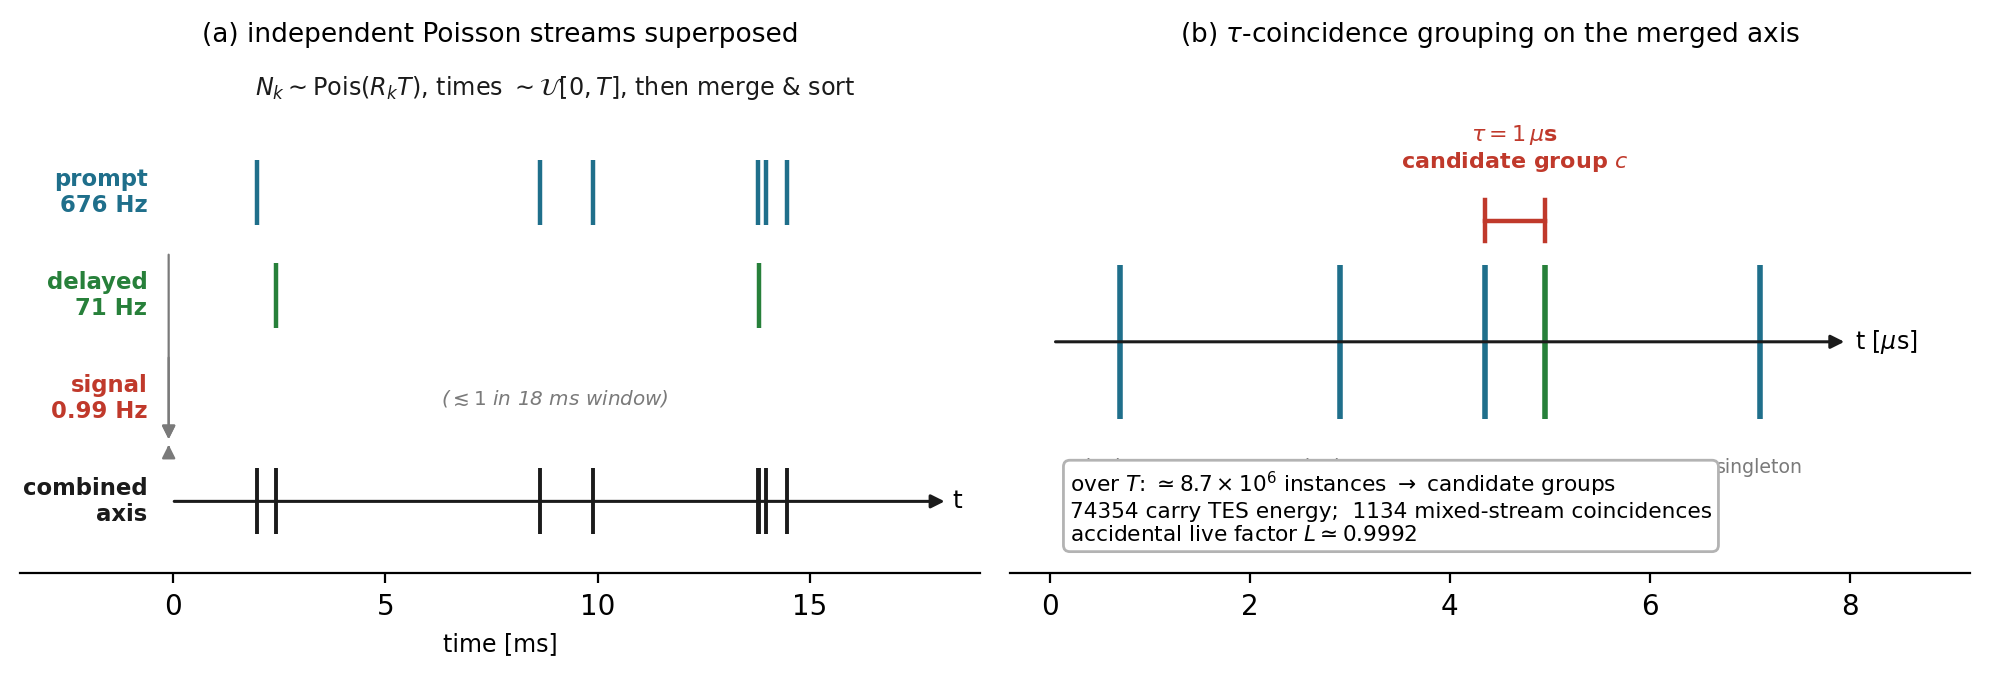
\includegraphics[width=\linewidth]{paper_source_figure_table/fig_s33_poisson_normalization.png}
\caption{Rate normalization on a common coincidence time axis. (a)~Full-band detector event rates ($928$, $97.1$, and $0.987\,\mathrm{s^{-1}}$). (b)~Independent Poisson draws of the three streams are merged and time-ordered; color marks stream identity and hatched bands mark each event's temporal footprint. (c)~Events with $\Delta t\le\tau=1\,\mu\mathrm{s}$ form one candidate group; the box gives the reference-exposure accidental bookkeeping. Tick positions are schematic.}
\label{fig:s33_poisson}
\end{figure}

\begin{figure}[t]
\centering
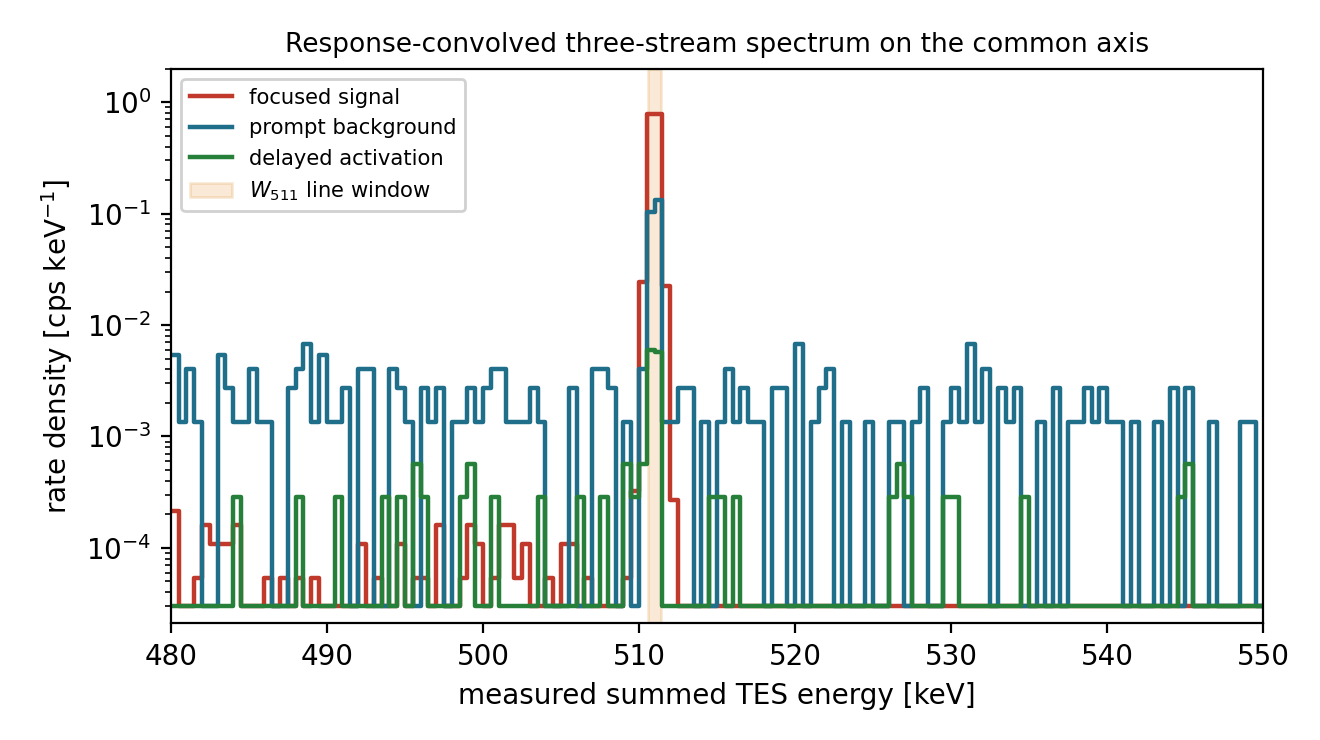
\includegraphics[width=0.72\linewidth]{paper_source_figure_table/fig_s33_spectrum_normalized.png}
\caption{Normalized summed-energy spectrum of the three streams on the common axis (raw stage). The focused signal, prompt, and delayed streams all concentrate at the 511\keV{} line while the continuum is starved. Shape-diagnostic re-derivation on the surviving Mass\_model\_511 catalogues; absolute selected rates are authoritative in Table~\ref{tab:phase2_cutflow}.}
\label{fig:s33_spec_norm}
\end{figure}

This post-processing superposition, rather than the native trigger/veto flags
present in the geometry description, defines the rate for two reasons. First,
both veto layers are defined by time coincidence: the active anticoincidence
gate compares the TES and active-shield deposits within the same $\tau$ window,
and the topology reconstruction must first decide which hits belong to the same
incident photon; both require a common time axis carrying all three streams at
their physical rates. Second, the common post-processing definition forces the
prompt, delayed, and focused-signal streams through the same coincidence window
$\tau$ and the same shield threshold, so that production-stage trigger flags do
not silently become the rate definition. The superposition is licensed by a
stationarity assumption: within the adopted reference exposure each stream rate
is treated as constant. The reference window is short compared with the
timescales over which the physical rates drift---the atmospheric column and the
activation inventory evolve on the mission-day scale, whereas on the
microsecond-to-second scale relevant to coincidence the three rates are
effectively stationary. A constant-rate arrival process is a homogeneous Poisson
process, and the superposition of independent homogeneous Poisson processes is
again Poisson with rate $\sum_k R_k$, which is exactly what licenses drawing
$N_k\sim\mathrm{Pois}(R_k T)$ and merging. The mission-time significance accordingly uses the expectation values of
these rates rather than adding a fresh random draw to every mission bin; the
Poisson realization only validates the grouping and accidental-coincidence
bookkeeping.

\subsubsection{Active anticoincidence gate}

The first layer is an active anticoincidence gate on this common time axis. For
each candidate group $c$ the TES and active-shield energy sums are
\begin{equation}
  E_{\mathrm{TES}}^{(c)}=\sum_{j\in c}E_{\mathrm{TES},j},\qquad
  E_{\mathrm{sh}}^{(c)}=\sum_{j\in c}E_{\mathrm{sh},j}.
\end{equation}
The group enters the hard line window if $E_{\mathrm{TES}}^{(c)}$ falls in
\begin{equation}
  \wii = [510.58,511.42]\keV \quad (511\keV\pm420\,\mathrm{eV}),
\end{equation}
which is the current Mass\_model\_511 selection window, retaining most of the line response while
suppressing continuum background. The group passes the active shield if
\begin{equation}
  E_{\mathrm{sh}}^{(c)} < E_{\mathrm{veto}}, \qquad E_{\mathrm{veto}}=50\keV,
\end{equation}
where for the baseline CsI configuration the shield sum is read from the CsI
active-shield volumes in post-processing. This layer is the dominant source of
rate-level background suppression. In the baseline it reduces the prompt background from 153 to 71 events ($0.1180\to0.0482\cps$, $40.8\%$ surviving) and the delayed activation from 43 to 28 events ($65.1\%$), while retaining all 30305 focused-signal events (zero shield deposit, $100\%$); see Table~\ref{tab:phase2_cutflow}. Its effect on the background spectrum is shown in Figure~\ref{fig:s33_spec_anti}.

\begin{figure}[t]
\centering
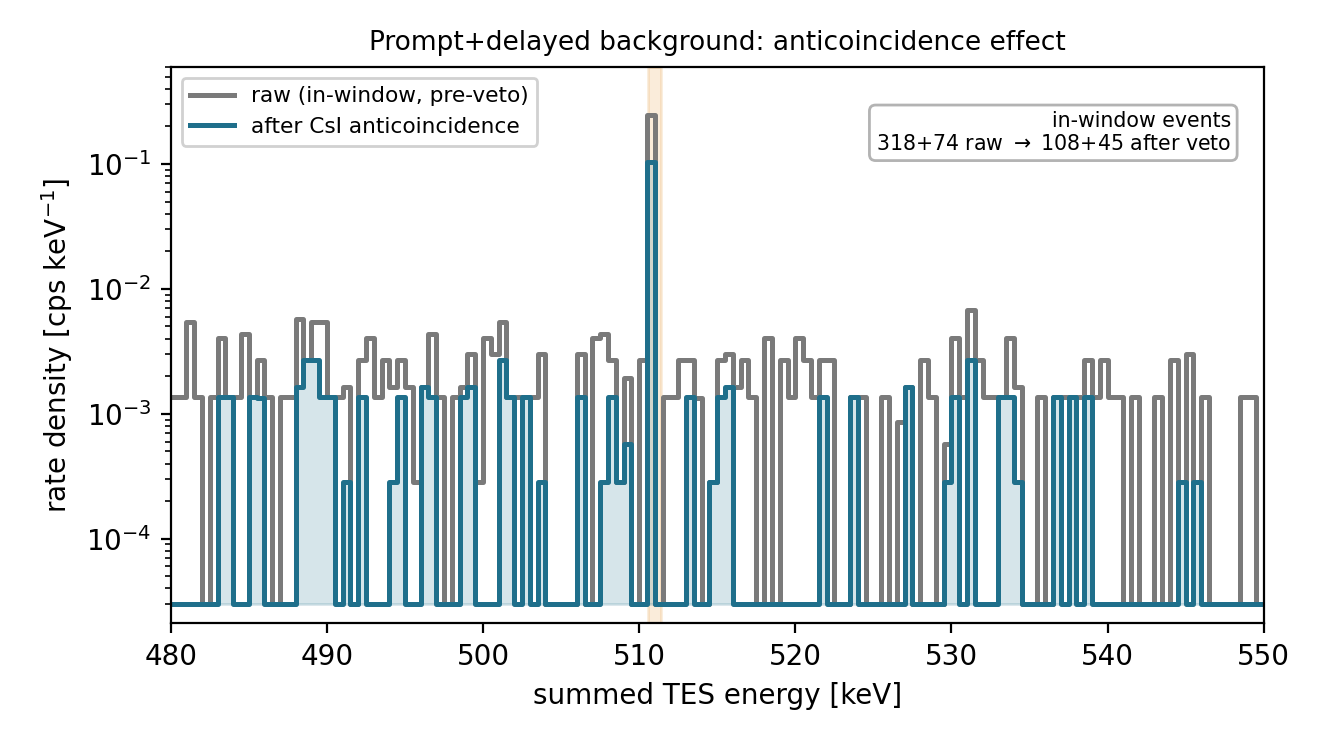
\includegraphics[width=0.72\linewidth]{paper_source_figure_table/fig_s33_spectrum_anticoincidence.png}
\caption{Effect of the CsI anticoincidence gate on the prompt$+$delayed background spectrum (in-window pre-veto vs after the shield gate). Shape-diagnostic re-derivation on the surviving Mass\_model\_511 catalogues.}
\label{fig:s33_spec_anti}
\end{figure} The quoted flux thresholds apply to a line
whose intrinsic width, after detector response, remains small compared with this
window; a substantially broadened source line would require convolving the
source line profile with the response and re-optimizing the window.

\subsubsection{Compton topology and field-of-view consistency}

The second layer applies a Compton-kinematic topology and field-of-view
consistency test to the TES hits that survive the active-shield gate; its
physical basis is Compton-camera cone reconstruction \cite{Zoglauer2006}. An
incident photon of energy $E_0$ Compton-scatters at a first interaction point
$\mathbf r_1$, depositing $E_1$, and the scattered photon of energy
$E_{\mathrm{sc}}=E_0-E_1$ propagates to a second interaction point $\mathbf r_2$;
the scattering angle follows from
\begin{equation}
  \cos\theta_C =
  1 - m_ec^2\left(\frac{1}{E_{\mathrm{sc}}}
  - \frac{1}{E_1+E_{\mathrm{sc}}}\right).
\end{equation}
Given the scattered-photon direction
$\hat{\mathbf u}_{12}=(\mathbf r_2-\mathbf r_1)/|\mathbf r_2-\mathbf r_1|$, the
source direction is constrained to a reconstruction cone with apex $\mathbf r_1$,
axis $-\hat{\mathbf u}_{12}$, and half-angle $\theta_C$, whose projection on the
sky is the event circle. This work does not perform imaging; it only tests
whether this first-scatter cone intersects the side Be-window disk (radius
$1.898\,\mathrm{cm}$), i.e.\ whether the reconstructed arrival direction is
consistent with entry through the aperture.

Because the interaction position within a single TES pixel
($1.5\times1.5\times3.0\,\mathrm{mm}$) is unresolved, each hit is represented not
by its centroid alone but by $8+1=9$ representative points---the eight pixel
corners and the centroid---carrying the sub-pixel position uncertainty
explicitly into the geometric reconstruction. A two-hit event in a given scatter
order therefore enumerates $9\times9=81$ first/second position combinations and
constructs one reconstruction cone per combination (each cone sampled at 24
azimuths, propagated to the Be-window plane, and tested against the disk by both
its sampled points and the connecting segments); the order is deemed
field-of-view consistent if any of these 81 trajectories yields a cone that
intersects the disk. This is a deliberately permissive consistency test: an
event is retained if any sub-pixel interaction position is consistent with entry
through the aperture. The layer consequently retains about $95\%$ of the
in-window multi-hit events and removes only about $10$--$14\%$ of the background,
consistent with its role as a loose consistency veto rather than an imaging
reconstruction.

The three event classes are handled accordingly. Single-pixel events have no
scatter topology and are retained as calorimetric line candidates. A two-hit
event provides two positions and energies but no internal information to order
the interactions, so both scatter orders are enumerated over the 81 trajectories
above, and the event is retained if either order is field-of-view consistent and
rejected only if neither order admits any kinematically valid cone. Three-hit
and higher-multiplicity events contain internal scatter vertices and can be
ordered from geometric--kinematic consistency: at each internal vertex the
scattering angle can be obtained both from the deposited energies through the
Compton formula and from the angle between successive flight directions, and the
two should agree for the correct order. All orders are enumerated (up to six TES
hits; higher multiplicities are retained without ordering), the best order
minimizes the Compton sequence residual
\begin{equation}
  Q = \sum_{i=1}^{n-2}
  \left(\cos\theta_{C,i} -
  \hat{\mathbf u}_{i-1,i}\cdot\hat{\mathbf u}_{i,i+1}\right)^2
\end{equation}
(ties broken by the longest first-scatter lever arm), and the same 81-trajectory
cone--disk test is applied to its first two points. Events with no valid order
are classified as unreconstructed. In the baseline, events that pass the active shield are sorted by the topology test into single-site, field-of-view-consistent reconstructed multi-hit, and vetoed classes: the prompt stream comprises 43 single-site, 22 reconstructed multi-hit, and 6 vetoed events (71 total); the delayed stream 20, 8, and 0 (28 total); and the focused signal 17589 single-site, 12098 reconstructed multi-hit, and 618 vetoed events (30305 total), giving 65, 28, and 29687 selected events, respectively. Reclassifying the current Mass\_model\_511 detector geometry in the $480$--$550\,\keV$ broad band by TES hit multiplicity (Figure~\ref{fig:s33_compton_mult}; shape diagnostic only; absolute selected rates remain those in Table~\ref{tab:phase2_cutflow}) resolves the selected focused-signal groups into 17598 single-site, 9794 two-hit, and 2340 $\geq$3-hit events (with 370 two-hit and 262 $\geq$3-hit events Compton-vetoed); multi-hit counts in the prompt and delayed streams remain small (two-/$\geq$3-hit: 25/7 and 12/3).

\begin{figure}[t]
\centering
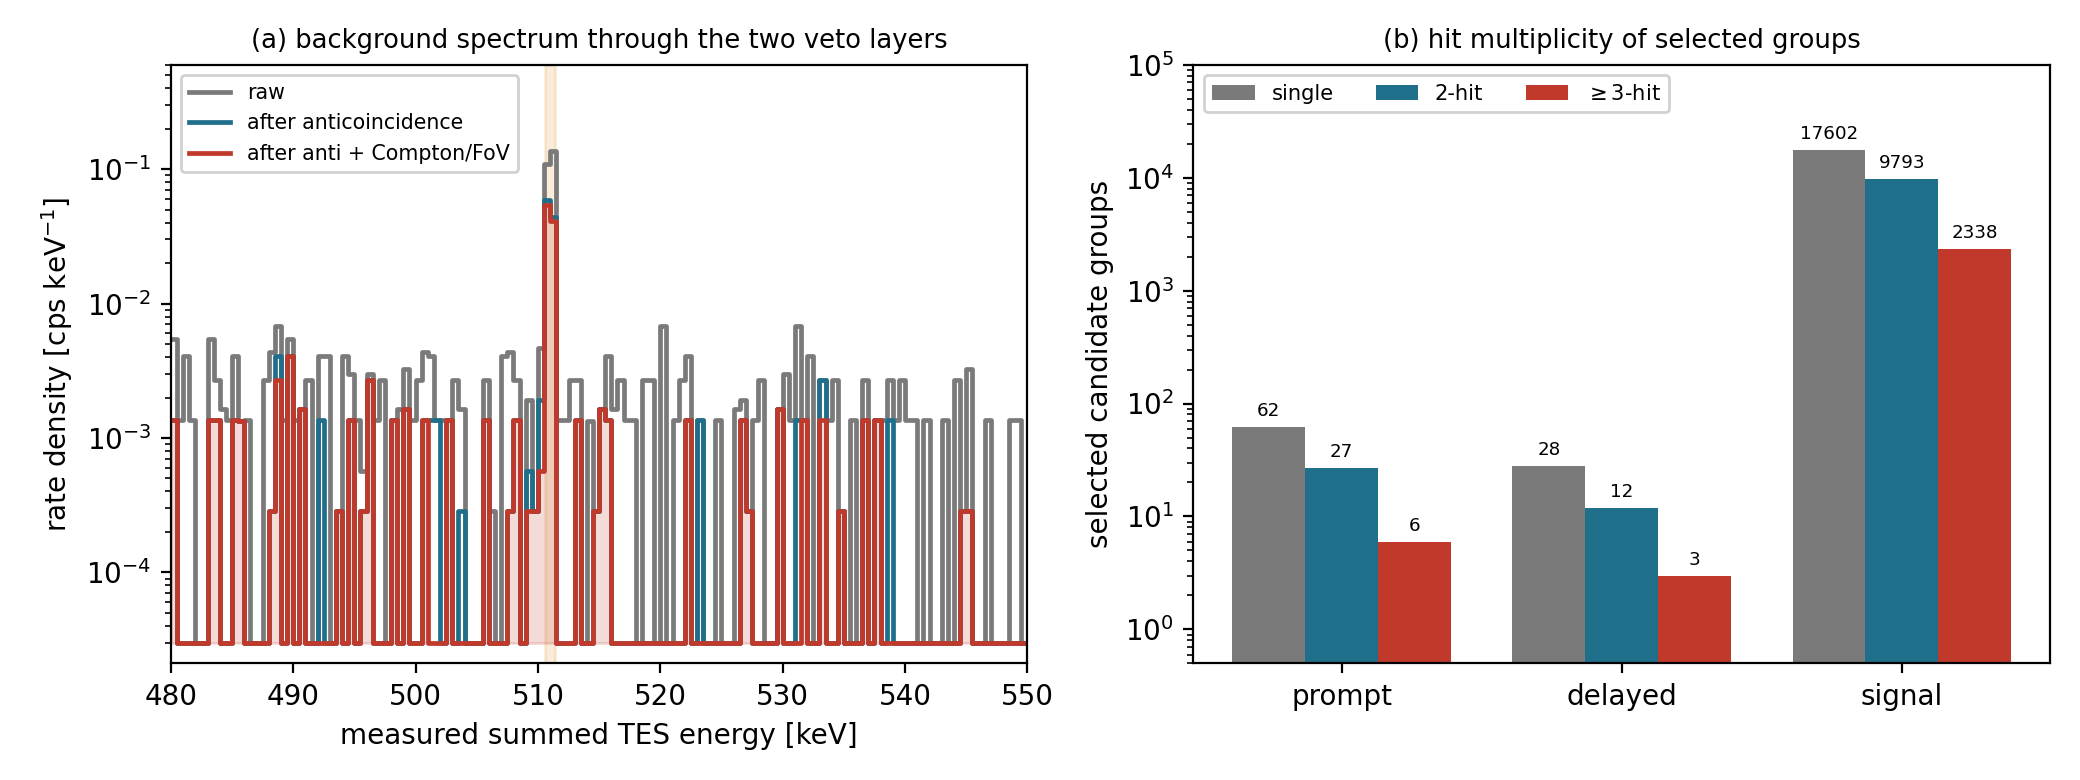
\includegraphics[width=\linewidth]{paper_source_figure_table/fig_s33_compton_multiplicity.png}
\caption{(a) Background spectrum through the two veto layers (raw; after anticoincidence; after anticoincidence$+$Compton/FoV). (b) Hit multiplicity of the selected candidate groups per stream. Shape-diagnostic re-derivation on the surviving Mass\_model\_511 catalogues; absolute rates are authoritative in Table~\ref{tab:phase2_cutflow}.}
\label{fig:s33_compton_mult}
\end{figure}

Unreconstructed events are retained in the baseline selected-rate definition but
are not counted as field-of-view passing, so the line-window result does not gain
sensitivity by discarding ambiguous reconstruction failures. This policy is also
not a conservative lower bound on the net sensitivity: a single-site-only
alternative that vetoes all multi-hit candidates would retain $59.2\%$ of the
focused signal ($17589/29687$) and about $66.6\%$ of the selected background in
the present $\wii$ sample, reducing the simple $S/\sqrt{B}$ figure to about
$0.73$ of the baseline value. The baseline selection therefore treats ambiguous
multi-hit events as a reconstruction-model boundary to be validated, not as a
source of sensitivity gain from aggressive event rejection.

\added{To connect this selection chain explicitly to the finite Monte Carlo
sample, Table~\ref{tab:phase2_cutflow} gives the current event-level
$\wii$ cut-flow obtained by lightweight replay of the simulated event catalogues.
The table is not a new Geant4/MEGAlib transport. It replays the current
event catalogues with the same TES energy window, CsI veto, and
Compton-kinematic/field-of-view consistency checks; uncertainties are Monte
Carlo quadrature sums over event weights. The current event-selection records first fix
the energy window and then report raw, active-shield, and topology stages, so
the raw stage should be read as the pre-veto sample inside the line window, not
as an all-energy incident sample.}

\begin{table}[t]
\centering
\caption{\added{event-level $\wii$ line-window cut-flow.}}
\label{tab:phase2_cutflow}
\footnotesize
{
\setlength{\tabcolsep}{3pt}
\begin{tabular}{p{0.20\linewidth}p{0.24\linewidth}p{0.08\linewidth}p{0.16\linewidth}p{0.20\linewidth}}
\toprule
Stream & Stage & Events & Rate / $\cps$ & Statistical uncertainty / $\cps$ \\
\midrule
Prompt background & Line-window pre-veto & 153 & $1.1802\times10^{-1}$ & $1.25\times10^{-2}$ \\
Prompt background & After CsI veto & 71 & $4.8160\times10^{-2}$ & $5.72\times10^{-3}$ \\
Prompt background & Topology/FOV selected & 65 & $4.4089\times10^{-2}$ & $5.47\times10^{-3}$ \\
Delayed activation & Line-window pre-veto & 43 & $6.1192\times10^{-3}$ & $9.33\times10^{-4}$ \\
Delayed activation & After CsI veto & 28 & $3.9846\times10^{-3}$ & $7.53\times10^{-4}$ \\
Delayed activation & Topology/FOV selected & 28 & $3.9846\times10^{-3}$ & $7.53\times10^{-4}$ \\
Focused signal & Line-window pre-veto & 30305 & $8.1478\times10^{-1}$ & $4.68\times10^{-3}$ \\
Focused signal & After CsI veto & 30305 & $8.1478\times10^{-1}$ & $4.68\times10^{-3}$ \\
Focused signal & Topology/FOV selected & 29687 & $7.9817\times10^{-1}$ & $4.63\times10^{-3}$ \\
\bottomrule
\end{tabular}
\par}
\vspace{0.5ex}
\begin{minipage}{0.94\linewidth}
\footnotesize
The focused-signal rows are unit-replay rates used to show veto survival
behavior; the point-source signal rate in Table~\ref{tab:primary_sensitivity}
is scaled separately by the Laue effective area, reference flux, and atmospheric
transmission.
\end{minipage}
\end{table}

As a retained reference-geometry cross-check that has not been rerun for
Mass\_model\_511, the focused-signal replay stream was
reconstructed with the MEGAlib revan Compton event reconstructor (37,065 events
processed, reading the existing simulation without re-running transport)
\cite{Zoglauer2006}. The class-level results agree with the custom chain:
in-window single-pixel events number 17,695 (revan) versus 17,663 (custom
chain), a $0.2\%$ difference, while the $3.2\%$ difference in the in-window total
(31,295 versus 30,323) follows from revan applying a per-hit Gaussian energy
response and a trigger threshold that feed the partial-absorption shoulder below
the window into it, predominantly in the multi-hit class, whereas the custom
chain takes the window on unnoised summed energies. For two-hit ordering the
cross-check gives two quantitative results. First, the fraction of two-hit
events with at least one kinematically valid order is $100.0\%$
($10{,}421/10{,}421$), as expected analytically---for a fully absorbed
$511\keV$ two-hit event the scattered-photon energy cannot fall below the
$E_0/3$ Compton edge, so at least one order is always valid---confirming the
premise for retaining two-hit events. Second, the best order chosen by the
Klein--Nishina cross section with a kinematic quality factor agrees with the
order that points more nearly toward the source only $78.4\%$ of the time, so
committing to a single estimated order (as an imaging chain would) would use the
wrong Compton cone for about $22\%$ of two-hit events, whereas enumerating both
orders and accepting either field-of-view-consistent one avoids this
misassignment. The cross-check also yields a quantitative bound absent from the
earlier chain: the median $|\mathrm{ARM}|$ of in-window Compton events relative
to the true beam direction is about $24^\circ$ (two-hit $23.6^\circ$; three-hit
and higher $26.3^\circ$; only about $32\%$ have $|\mathrm{ARM}|<10^\circ$),
driven by the millimetre-scale scatter lever arms and pixel quantization; this
explains why the topology/field-of-view layer removes only about $10$--$14\%$ of
the background and cannot be sharpened into an imaging-level discriminant.
Finally, the fraction of unorderable events is very small (61 of 37,065, i.e.\
$0.16\%$, in revan; one in the custom chain), showing that the unreconstructed
class is a small boundary population rather than a hidden pillar of the
sensitivity.

81 points from 0 to 20 d with 0.25 d spacing; endpoint points carry half-widths
in the count integration. The trajectory is a synthetic reference profile, not
balloon telemetry. For time-grid point $t_i$ in days,
\begin{align}
  h_i &= h_0+\Delta h\sin\!\left[\frac{2\pi(t_i-15)}{5}\right],\\
  \varphi_i &= \varphi_0+\Delta\varphi\sin\!\left[\frac{2\pi(t_i-15)}{7}\right],\\
  \ell_i &= \ell_0+\Delta\ell\sin\!\left[\frac{2\pi(t_i-15)}{9}\right],
\end{align}
where $h_0=38.75\,\mathrm{km}$, $\Delta h=2.5\,\mathrm{km}$,
$\varphi_0=34^\circ$, $\Delta\varphi=0.25^\circ$, $\ell_0=100^\circ$,
and $\Delta\ell=0.25^\circ$. The resulting ranges are
$36.25$--$41.25\,\mathrm{km}$ in altitude, $33.75^\circ$--$34.25^\circ$ in
latitude, and $99.75^\circ$--$100.25^\circ$ in longitude.

The atmospheric depth and the 511 keV transmission scale are
\begin{align}
  X(h_i) &= X_{38}\exp\!\left[-\frac{h_i-38\,\mathrm{km}}{H}\right],
       & X_{38}&=3.87\,\mathrm{g\,cm^{-2}},\quad H=6.8\,\mathrm{km},\\
  T_i &= \exp[-\mu_{\mathrm{eff}} X(h_i)],
       & \mu_{\mathrm{eff}}&=-\frac{\ln T_{15}}{X(h_0)},
\end{align}
with $T_{15}=0.739$. Thus the focused-science scale is
$f_{\mathrm{atm},i}=T_i/T_{15}$. The prompt atmospheric source scale is
\begin{align}
  R_{c,i} &= 11.0 -0.08(\varphi_i-\varphi_0)+0.03(\ell_i-\ell_0),\\
  f_{\mathrm{p},i} &=
  \exp\!\left[\frac{X(h_i)-X(h_0)}{30\,\mathrm{g\,cm^{-2}}}\right]
  \left(\frac{11.0}{R_{c,i}}\right)^{0.2}.
\end{align}
The trajectory rigidity model is centered on a rounded value, and $f_{\mathrm{p},i}$ enters only through the day-15--anchored ratio $(11.0/R_{c,i})^{0.2}$, so this central value affects the mission-time variation but not the absolute prompt rate, which is fixed by the $R_c=11.6\,\mathrm{GV}$ source definition. The same scalar production driver is used for delayed activation before
isotope-by-isotope decay buildup is solved. For a delayed-production element
$a$ with decay constant $\lambda_a$ and fixed day-15 activity $A_{a,15}$,
\begin{align}
  P_{a,15} &= \frac{A_{a,15}}{1-\exp(-\lambda_a t_{15})},\\
  \frac{dN_a}{dt} &= P_{a,15}f_{\mathrm{p}}(t)-\lambda_a N_a,\qquad
  A_a(t)=\lambda_a N_a(t).
\end{align}
The numerical fold anchors the solution back to $A_{a,15}$ at day 15 and sums
the activity over the nuclide/material/position production elements.

This delayed-activity treatment assumes that the normalized activation-product
distribution is unchanged over the small trajectory range, and that the
trajectory changes only the scalar production driver. The verification
described here checks the internal implementation of that model but does not
prove physical invariance of the production distribution. If dedicated activation transports at the trajectory center and
extrema show material or nuclide redistribution, the scalar driver should be
replaced by interpolation over production vectors,
\begin{equation}
  P_a(t_i)=\sum_g w_g(h_i,\varphi_i,\ell_i,R_{c,i})P_a^{(g)},\qquad
  \sum_g w_g=1,
\end{equation}
followed by the same decay ODE.

Implementation checks recomputed the trajectory formula at the center point and
at the two altitude extrema. The reference atmospheric transmission is
$T=0.739$ at the day-15 anchor, and the high- and low-altitude probes give
$T=0.811$ and $0.646$, respectively. Reconstructing the $\wii$ prompt,
delayed, background, and signal rates from the day-15 rates and these scales
reproduces the mission-fold summary. Reweighting the particle families with local PARMA spectra at the same trajectory probes shifts the normalized nuclide--volume activity distribution by less than $6\times10^{-3}$ in total-variation distance. This supports using a scalar delayed
production/activity fold for the present small trajectory range at the
particle-family reweighting layer. It is not a full proof of distribution
invariance: same-particle energy/angle-dependent activation cross sections and
position-transport shifts would require dedicated low-, reference-, and
high-altitude activation-production transports.

In the mission-time fold, the selected day-15 rates are folded over the
trajectory grid as
\begin{align}
  B_i &= L_i\left(B_{\mathrm{p},15} f_{\mathrm{p},i}
        + B_{\mathrm{d},15} f_{\mathrm{d},i}\right),\\
  S_i &= L_i S_{15} f_{\mathrm{atm},i},\\
  L_i &= \exp[-(R_{\mathrm{p},i}+R_{\mathrm{d},i})\tau],
\end{align}
where $f_{\mathrm{p},i}$ is the prompt atmospheric scale,
$f_{\mathrm{d},i}$ is the delayed-activity scale, $f_{\mathrm{atm},i}$ is the
511 keV atmospheric transmission scale, and $L_i$ is the accidental
coincidence live factor. Here $R_{\mathrm{p},i}$ and $R_{\mathrm{d},i}$ are the
prompt and delayed event rates entering the coincidence grouping at that mission point. The factor $L_i$ assumes a one-sided $\tau$ gate; a symmetric $\pm\tau$ condition would instead give $\exp[-2(R_{\mathrm{p},i}+R_{\mathrm{d},i})\tau]$, but for the present rates both forms remain very close to unity, so the folded counts are insensitive to this choice.

The time-dependent significance is computed as a cumulative counting statistic. For a reference flux $\fzero$, the cumulative significance is
\begin{equation}
  Z(t_m) = \frac{N_s(t_m)}{\sqrt{N_b(t_m)}},
\end{equation}
where
\begin{equation}
  N_s(t_m)=\sum_{i\leq m}S_i\Delta t_i,\qquad
  N_b(t_m)=\sum_{i\leq m}B_i\Delta t_i
\end{equation}
are the time-integrated selected signal and background counts after
mission-time scaling and live-factor corrections. For comparison among
analysis variants, the $3\sigma$ flux threshold is scaled as
\begin{equation}
  \fthree(t_m) = \fzero \frac{3}{Z(t_m)}.
\end{equation}
This Gaussian counting convention is used consistently for the line-window
results and secondary comparisons, but it is a diagnostic selected-rate metric,
not a final flight discovery likelihood. For the present 20 d reference case,
the signal-to-background ratio is about 2.4\%; a 1\% Gaussian uncertainty on the
background normalization alone would reduce the approximate significance from
about 7.0 to about 2.3. A flight analysis would therefore require off-source
or control-band background constraints and nuisance-parameter profiling.
For the primary 20 d line-window result, the folded counts are about
$8.3\times10^4$ background counts and $2.0\times10^3$ signal counts at
$\fzero$, so this approximation is used only in the high-count selected-rate
regime. The isolated upstream Ge-proxy result with zero selected events is
reported separately with a Poisson zero-count upper limit.
The detector-selection summary also records a day-15 direct expectation. The primary
result does not use that constant-rate direct value; it uses the
mission-time fold and the final cumulative significance. The distinction is
small for the present line-window case, but keeping it explicit is necessary
for comparing analysis configurations.


\section{Results}
\label{sec:results}

The recovered log fragments around the original detailed results tables are structurally mixed. This compile-ready copy therefore keeps the confirmed primary selected-rate numbers in a compact recovery table and leaves the original detailed table reconstruction to manual editing.

\begin{table}[h]
\centering
\caption{Recovered primary unresolved-line selected-rate result.}
\label{tab:primary_sensitivity}
\begin{tabular}{lll}
\toprule
Quantity & Value & Note \\
\midrule
Day-15 selected background & $4.81\times10^{-2}\cps$ & Prompt + delayed \\
Day-15 selected signal at $\fzero$ & $1.18\times10^{-3}\cps$ & $\fzero=10^{-4}\phcms$ \\
Prompt background fraction & $91.7\%$ & Dominant component \\
20 d diagnostic $Z$ & $7.04$ & Counting metric \\
$\fthree(20\,\mathrm{d})$ & $4.26\times10^{-5}\phcms$ & Reference model only \\
\bottomrule
\end{tabular}
\end{table}

\clearpage
\section*{Recovery gap note}
The original recovered log fragments become structurally inconsistent after this point. The broad-window diagnostic paragraph and several nearby transition lines are omitted from this compile-ready reading copy; see the raw partial source and recovery manifest.

\section{Discussion and conclusions}
\label{sec:discussion}

The main result is that the reference production-position delayed-source calculation gives a 20 d diagnostic $3\sigma$ point-source threshold of $4.26\times10^{-5}\phcms$ for an unresolved line in the modeled focused TES line spectrometer. This threshold is obtained without using the focused-spot spatial analysis as the primary result. It follows from three combined effects: optical concentration, a sub-keV energy window, and a detector-coupled veto/topology selection that suppresses prompt and delayed backgrounds in the same selection space as the signal.

This calculation should be compared with existing 511 keV instruments as a pointed, narrow-line, compact-source estimate, not as an all-sky imaging forecast. INTEGRAL/SPI and COSI provide the reference measurements for mapping the diffuse 511 keV sky and the broader Galactic diffuse emission \cite{Siegert2016AA,Kierans2020,Siegert2020COSI,Yoneda2025,Karwin2023}. Peer-reviewed COSI calibration and simulation studies provide the more relevant technical comparison for detector response, event reconstruction, and balloon-background validation \cite{Beechert2022,Sleator2019,Gallego2025Balloon,Gallego2025,Ciabattoni2025ACS}. The TES Laue-lens concept considered here is complementary: it trades sky coverage for a concentrated beam and a sub-keV line window. The relevant comparison class is compact 511 keV targets, unresolved-central-excess searches, and transient follow-up observations with known or constrained source positions. The same focused aperture is not a substitute for measuring the full diffuse bulge and disk luminosity, because it samples only a small solid angle.

The production-position delayed-source treatment addresses a specific approximation in radial-profile compression. Although delayed activation contributes only about 8.3\% of the selected line-window background in the present calculation, it is spatially and materially structured. Preserving sampled production positions prevents artificial azimuthal or radial redistribution from becoming an unquantified systematic. The current Mass\_model\_511 result uses one full-stat production-position sampling; a same-statistics multi-seed selected-rate convergence check remains open.

The background composition indicates the first engineering parameters to test, rather than a completed optimization. The selected line-window rate remains dominated by prompt atmospheric streams, so shield geometry, side-entry collimation, material near the focal plane, topology selection, and multi-pixel reconstruction are the most direct handles on the present background. Delayed activation is smaller but remains spatially and materially structured, so source-position preservation is retained in the rate calculation. The dominance of iodine activation in the CsI shield also motivates a future shield-material trade study.

\subsection{Limitations and future validation}
\label{subsec:limitations}

\rewritten{The selected-rate result has five immediate boundaries. First, the detector/cryostat model is an engineering proxy, not a final flight CAD model. Second, quantitative active-shield rejection is applied in the common detector-level post-processing selection rather than by production-time trigger/veto filtering. Third, the mission-time calculation is a rate-level fold, not a new particle transport at each trajectory time bin. Fourth, the custom Compton/field-of-view veto is a detector-level topology and kinematic consistency check, not yet a full Revan/Mimrec reconstruction, and the retained reconstruction-failure class is a baseline acceptance choice rather than a conservative sensitivity bound. Fifth, the event-level analysis has made the cut-flow, broad-window spectra, veto behavior, and activation selected-event decomposition traceable, but selected delayed state/metastable labels, the merged four-sampling per-event decomposition, post-veto energy-window staging, multi-pixel residual distributions, and veto-threshold stability scans are still not closed by the current outputs.}

More generally, the tabulated $3\sigma$ flux thresholds are statistical selected-rate thresholds for the reference source, mass, and response model. They do not include a systematic-uncertainty envelope for atmospheric-flux normalization, activation cross sections or physics-list choices, material and geometry tolerances, detector energy-response uncertainty, veto-threshold calibration, reconstruction-efficiency systematics, or background-estimation nuisance parameters. A publication-level flight sensitivity should replace the diagnostic $S/\sqrt{B}$ metric with a spatial-spectral likelihood, following standard profile-likelihood practice \cite{Cowan2011}.

The retained upstream Laue-lens calculation should be read as a boundary calculation for an equal-volume/equal-mass active-Ge proxy, not as a finalized optics-background budget. It completes full-particle prompt and activation-production transport for the proxy, and the isolated Ge-proxy delayed component gives zero selected $\wii$ events in the retained transport. The prompt self-background contribution is still not part of the primary detector-background budget because it needs source separation or subtraction from the ordinary detector/cryostat prompt background, and explicit lens support hardware is not yet modeled.

Spatial analyses such as $r_{90}$ and multi-annulus likelihood estimates are diagnostic cross-checks, but they are not yet a finalized nuisance-profile likelihood. The quoted sensitivity therefore remains the line-window selected-rate result, not a spatially optimized likelihood result.

\rewritten{Before this rate study can support a flight-performance statement, four validation blocks remain: a Revan/Mimrec or equivalent reconstruction cross-check of the retained multi-hit subset, including residual distributions and threshold stability; optics self-background transport with explicit lens tiles and support hardware at final statistics; a final cryostat/DR geometry and detector-response update, including TES saturation and pile-up constraints; and a spatial-spectral likelihood that profiles background nuisance parameters. The event-level tables added here should be read as manuscript support evidence and audit entry points before those validations, not as a complete systematic-uncertainty envelope.}

\subsection{Conclusions}
\label{sec:conclusions}

We have presented a detector-coupled background and sensitivity study for a balloon-borne pointed 511 keV TES Laue-lens telescope. The reference calculation couples a Ge(111) Laue optical response to a TES focal-plane mass model, prompt atmospheric transport, delayed activation, active-shield vetoing, topology/field-of-view selection, mission-time rate folding, and counting-significance evaluation. In the primary $510.58$--$511.42\keV$ unresolved-line window, the day-15 selected rates are $B\simeq4.81\times10^{-2}\cps$ and $S\simeq1.18\times10^{-3}\cps$ at $10^{-4}\phcms$; the mission-time fold gives $Z_{20\mathrm{d}}\simeq7.04$ and $\fthree(20\mathrm{d})\simeq4.26\times10^{-5}\phcms$. The result provides a detector-coupled selected-rate basis for continued evaluation of focused TES spectroscopy as a complementary 511 keV technique for compact-source and unresolved-central-excess searches, while identifying prompt atmospheric background suppression, delayed-activation systematic validation, and reconstruction validation as the main next validation tasks.

\section*{Data and software availability}
Before publication, a versioned public repository or institutional archive should provide the geometry and source definitions, random seeds, analysis and figure-generation scripts, LaTeX source, and derived validation products needed to reproduce the tables and figures in this paper. This compile-ready recovery copy is not the original final manuscript.

\section*{Declarations}
\textbf{Funding} To be completed before journal submission.

\textbf{Competing interests} To be completed before journal submission.

\textbf{Author contributions} To be completed before journal submission.

\textbf{Ethics approval and consent to participate} Not applicable.

\begin{thebibliography}{99}

\bibitem[Prantzos et~al.(2011)]{Prantzos2011}
N. Prantzos, C. Boehm, A.M. Bykov, R. Diehl, K. Ferriere, N. Guessoum, P. Jean, J. Knoedlseder, A. Marcowith, I.V. Moskalenko, A. Strong, G. Weidenspointner, The 511 keV emission from positron annihilation in the Galaxy, Rev. Mod. Phys. 83 (2011) 1001--1056, doi:10.1103/RevModPhys.83.1001.

\bibitem[Jean et~al.(2006)]{Jean2006}
P. Jean, J. Knoedlseder, V. Lonjou, M. Allain, J.-P. Roques, G.K. Skinner, B.J. Teegarden, G. Vedrenne, P. von Ballmoos, B. Cordier, P. Caraveo, R. Diehl, P. Durouchoux, P. Leleux, R. Schanne, G. Weidenspointner, Spectral analysis of the Galactic $e^+e^-$ annihilation emission, Astron. Astrophys. 445 (2006) 579--589, doi:10.1051/0004-6361:20053765.

\bibitem[Siegert et~al.(2016)]{Siegert2016AA}
T. Siegert, R. Diehl, G. Khachatryan, M.G.H. Krause, F. Guglielmetti, J. Greiner, A.W. Strong, X. Zhang, Gamma-ray spectroscopy of positron annihilation in the Milky Way, Astron. Astrophys. 586 (2016) A84, doi:10.1051/0004-6361/201527510.

\bibitem[Siegert et~al.(2019)]{Siegert2019Kinematics}
T. Siegert, R. Diehl, G. Khachatryan, M.G.H. Krause, F. Guglielmetti, J. Greiner, A.W. Strong, X. Zhang, Constraints on positron annihilation kinematics in the inner Galaxy, Astron. Astrophys. 627 (2019) A126, doi:10.1051/0004-6361/201833856.

\bibitem[Yoneda et~al.(2025)]{Yoneda2025}
H. Yoneda, T. Siegert, S. Mittal, Imaging the positron annihilation line with 20 years of INTEGRAL/SPI observations, arXiv:2509.01066, 2025.

\bibitem[Kierans et~al.(2020)]{Kierans2020}
C.A. Kierans, S.E. Boggs, A. Zoglauer, A.W. Lowell, C. Sleator, J. Beechert, T.J. Brandt, P. Jean, H. Lazar, J. Roberts, T. Siegert, J.A. Tomsick, P. von Ballmoos, Detection of the 511 keV Galactic positron annihilation line with COSI, Astrophys. J. 895 (2020) 44, doi:10.3847/1538-4357/ab89a9.

\bibitem[Siegert et~al.(2020)]{Siegert2020COSI}
T. Siegert, S.E. Boggs, J.A. Tomsick, A.C. Zoglauer, C.A. Kierans, C.C. Sleator, J. Beechert, T.J. Brandt, P. Jean, H. Lazar, A.W. Lowell, J.M. Roberts, P. von Ballmoos, Imaging the 511 keV positron annihilation sky with COSI, Astrophys. J. 897 (2020) 45, doi:10.3847/1538-4357/ab9607.

\bibitem[Knoedlseder et~al.(2005)]{Knodlseder2005AllSky}
J. Knoedlseder, P. Jean, V. Lonjou, G. Weidenspointner, N. Guessoum, R. Diehl, W. Gillard, M.J. Harris, G.K. Skinner, P. von Ballmoos, G. Vedrenne, P. Caraveo, B. Cordier, V. Schoenfelder, B.J. Teegarden, The all-sky distribution of 511 keV electron-positron annihilation emission, Astron. Astrophys. 441 (2005) 513--532, doi:10.1051/0004-6361:20042063.

\bibitem[De Cesare(2011)]{DeCesare2011}
G. De Cesare, Searching for the 511 keV annihilation line from galactic compact objects with the IBIS gamma ray telescope, Astron. Astrophys. 531 (2011) A56, doi:10.1051/0004-6361/201116516.

\bibitem[Shirazi et~al.(2023)]{Shirazi2023}
F. Shirazi, E. Gau, M.A. Hossen, D. Becker, D. Schmidt, D. Swetz, D. Bennett, D. Braun, F. Kislat, J. Gard, J. Mates, J. Weber, N.R. Cavero, S. Chun, L. Lisalda, A. West, B. Dev, F. Ferrer, R. Bose, J. Ullom, H. Krawczynski, The 511-CAM Mission: A pointed 511 keV gamma-ray telescope with a focal plane detector made of stacked transition edge sensor microcalorimeter arrays, J. Astron. Telesc. Instrum. Syst. 9 (2023) 024006, doi:10.1117/1.JATIS.9.2.024006.

\bibitem[Barriere et~al.(2009)]{Barriere2009Laue}
N.M. Barriere, L. Natalucci, N. Abrosimov, P. von Ballmoos, P. Bastie, P. Courtois, M. Jentschel, J. Knodlseder, J. Rousselle, P. Ubertini, Soft gamma-ray optics: new Laue lens design and performance estimates, arXiv:0910.0488, 2009.

\bibitem[Barriere et~al.(2011)]{Barriere2011LauePrototype}
N.M. Barriere, J.A. Tomsick, S.E. Boggs, A. Lowell, P. von Ballmoos, Developing a second generation Laue lens prototype: high reflectivity crystals and accurate assembly, arXiv:1111.6700, 2011.

\bibitem[Weidenspointner et~al.(2006)]{Weidenspointner2006MAX}
G. Weidenspointner, C.B. Wunderer, N. Barriere, A. Zoglauer, P. von Ballmoos, Monte Carlo study of detector concepts for the MAX Laue Lens gamma-ray telescope, arXiv:astro-ph/0603152, 2006.

\bibitem[Sanchez del Rio \& Dejus(2011)]{SanchezDelRio2011XOP}
M. Sanchez del Rio, R.J. Dejus, XOP v2.4: recent developments of the x-ray optics software toolkit, Proc. SPIE 8141 (2011) 814115, doi:10.1117/12.893911.

\bibitem[Guan et~al.(2023)]{Guan2023BraggReflection}
F. Guan, M. Asai, D.A. Bartkoski, M. Kleckner, Z. Harel, M. Salehpour, Adding the X-ray Bragg reflection physical process in crystal to the Geant4 Monte Carlo simulation toolkit, part I: reflection from a crystal slab, Precision Radiation Oncology 7(1) (2023) 59--66.

\bibitem[Reiazi et~al.(2025)]{Reiazi2025G4BraggReflection}
R. Reiazi, D. Lee, D. Bartkoski, M. Kleckner, M. Salehpour, G4BraggReflection for accurate modeling of Bragg reflection in perfect and mosaic crystals, J. Phys. D: Appl. Phys. 58 (2025) 295102, doi:10.1088/1361-6463/aded1d.

\bibitem[Siegert et~al.(2016)]{Siegert2016V404}
T. Siegert, R. Diehl, J. Greiner, M.G.H. Krause, A.M. Beloborodov, M. Cadolle Bel, F. Guglielmetti, J. Rodriguez, A.W. Strong, X. Zhang, Positron annihilation signatures associated with the outburst of the microquasar V404 Cygni, Nature 531 (2016) 341--343, doi:10.1038/nature16978.

\bibitem[Gottardi \& Nagayoshi(2021)]{Gottardi2021TESReview}
L. Gottardi, K. Nagayoshi, A review of X-ray microcalorimeters based on superconducting transition edge sensors for astrophysics and particle physics, Applied Sciences 11 (2021) 3793, doi:10.3390/app11093793.

\bibitem[Xie et~al.(2026)]{Xie2026AlMn}
L. Xie, Y. Zhang, Z. Li, Z. Liu, S. Shu, J. Zhou, X. Li, H. Li, H. Gao, Y. Gu, X. Lu, Y. Zhao, C. Liu, Beyond one-thousandth energy resolution with an AlMn TES detector, arXiv:2602.11728, 2026.

\bibitem[Vavagiakis et~al.(2017)]{Vavagiakis2017AlMnMagnetic}
E.M. Vavagiakis, S.W. Henderson, K. Zheng, H.-M. Cho, N.F. Cothard, B. Dober, S.M. Duff, P.A. Gallardo, G. Hilton, J. Hubmayr, K.D. Irwin, B.J. Koopman, D. Li, F. Nati, M.D. Niemack, C.D. Reintsema, S. Simon, J.R. Stevens, A. Suzuki, B. Westbrook, Magnetic sensitivity of AlMn TESes and shielding considerations for next-generation CMB surveys, arXiv:1710.08456, 2017.

\bibitem[Hubbell \& Seltzer]{NISTXCOM}
J.H. Hubbell, S.M. Seltzer, XCOM: Photon Cross Section Database, NIST Standard Reference Database 8 (XGAM), National Institute of Standards and Technology, doi:10.18434/T48G6X.

\bibitem[Zhang et~al.(2022)]{Zhang2022TESGamma}
S. Zhang, J.-K. Xia, T. Sun, et al., Transition edge sensor based detector: from X-ray to gamma-ray, arXiv:2204.00010, 2022.

\bibitem[Gehrels(1985)]{Gehrels1985}
N. Gehrels, Instrumental background in balloon-borne gamma-ray spectrometers and techniques for its reduction, Nucl. Instrum. Methods Phys. Res. A 239 (1985) 324--349, doi:10.1016/0168-9002(85)90732-6.

\bibitem[Sato(2015)]{Sato2015EXPACS}
T. Sato, Analytical model for estimating terrestrial cosmic ray fluxes nearly anytime and anywhere in the world: extension of PARMA/EXPACS, PLoS ONE 10 (2015) e0144679, doi:10.1371/journal.pone.0144679.

\bibitem[Sato(2016)]{Sato2016PARMA4}
T. Sato, Analytical model for estimating the zenith angle dependence of terrestrial cosmic ray fluxes, PLoS ONE 11 (2016) e0160390, doi:10.1371/journal.pone.0160390.

\bibitem[Kondev et~al.(2021)]{Kondev2021NUBASE}
F.G. Kondev, M. Wang, W.J. Huang, S. Naimi, G. Audi, The NUBASE2020 evaluation of nuclear physics properties, Chinese Phys. C 45 (2021) 030001, doi:10.1088/1674-1137/abddae.

\bibitem[Sturner et~al.(2003)]{Sturner2003}
S.J. Sturner, C.R. Shrader, G. Weidenspointner, B.J. Teegarden, D. Attie, B. Cordier, R. Diehl, C. Ferguson, P. Jean, A. von Kienlin, P. Paul, F. Sanchez, S. Schanne, P. Sizun, G. Skinner, C.B. Wunderer, Monte Carlo simulations and generation of the SPI response, Astron. Astrophys. 411 (2003) L81--L84, doi:10.1051/0004-6361:20031171.

\bibitem[Agostinelli et~al.(2003)]{Agostinelli2003}
S. Agostinelli, J. Allison, K. Amako, et al., Geant4---a simulation toolkit, Nucl. Instrum. Methods Phys. Res. A 506 (2003) 250--303, doi:10.1016/S0168-9002(03)01368-8.

\bibitem[Allison et~al.(2016)]{Allison2016}
J. Allison, K. Amako, J. Apostolakis, et al., Recent developments in Geant4, Nucl. Instrum. Methods Phys. Res. A 835 (2016) 186--225, doi:10.1016/j.nima.2016.06.125.

\bibitem[Zoglauer et~al.(2006)]{Zoglauer2006}
A. Zoglauer, R. Andritschke, F. Schopper, MEGAlib: The Medium Energy Gamma-ray Astronomy Library, New Astron. Rev. 50 (2006) 629--632, doi:10.1016/j.newar.2006.06.049.

\bibitem[Caputo et~al.(2017)]{Caputo2017}
R. Caputo, F. Kislat, J. Racusin, on behalf of the AMEGO Team, AMEGO: Simulations of the instrument performance, Proc. 35th International Cosmic Ray Conference, PoS(ICRC2017) 783 (2018), doi:10.22323/1.301.0783.

\bibitem[Karwin et~al.(2023)]{Karwin2023}
C.M. Karwin, T. Siegert, J. Beechert, J.A. Tomsick, T.A. Porter, M. Negro, C. Kierans, M. Ajello, I. Martinez Castellanos, A. Shih, A. Zoglauer, S.E. Boggs, Probing the Galactic diffuse continuum emission with COSI, arXiv:2310.12206, 2023.

\bibitem[Gallego et~al.(2025a)]{Gallego2025Balloon}
S. Gallego, U. Oberlack, J. Lommler, C.M. Karwin, A. Zoglauer, P. Jean, P. von Ballmoos, C. Kierans, C.C. Sleator, J.A. Tomsick, S.E. Boggs, Bottom-up background simulations of the 2016 COSI balloon flight, arXiv:2503.02493, 2025.

\bibitem[Gallego et~al.(2025b)]{Gallego2025}
S. Gallego, U. Oberlack, J. Lommler, C.M. Karwin, F. Fenu, V. Fioretti, A. Zoglauer, et al., Pre-flight background estimates for COSI, arXiv:2510.25304, 2025.

\bibitem[Beechert et~al.(2022)]{Beechert2022}
J. Beechert, H. Lazar, S.E. Boggs, T.J. Brandt, Y.-C. Chang, C.-Y. Chu, H. Gulick, C. Kierans, A. Lowell, N. Pellegrini, J.M. Roberts, T. Siegert, C.C. Sleator, J.A. Tomsick, A. Zoglauer, Calibrations of the Compton Spectrometer and Imager, Nucl. Instrum. Methods Phys. Res. A 1031 (2022) 166510, doi:10.1016/j.nima.2022.166510.

\bibitem[Sleator et~al.(2019)]{Sleator2019}
C.C. Sleator, A. Zoglauer, A.W. Lowell, C.A. Kierans, S.E. Boggs, J.A. Tomsick, H. Lazar, J. Beechert, T.J. Brandt, P. von Ballmoos, Benchmarking simulations of the Compton Spectrometer and Imager with calibrations, Nucl. Instrum. Methods Phys. Res. A 946 (2019) 162643, doi:10.1016/j.nima.2019.162643.

\bibitem[Ciabattoni et~al.(2025)]{Ciabattoni2025ACS}
A. Ciabattoni, V. Fioretti, J.A. Tomsick, A. Zoglauer, P. Patel, L. Mitchell, A. Bulgarelli, P. Jean, G. Panebianco, N. Parmiggiani, C. Vignali, P. von Ballmoos, E. Wulf, Benchmarking of Geant4 simulations for the COSI anticoincidence system, Experimental Astronomy (2025), doi:10.1007/s10686-025-10019-7.

\bibitem[Cowan et~al.(2011)]{Cowan2011}
G. Cowan, K. Cranmer, E. Gross, O. Vitells, Asymptotic formulae for likelihood-based tests of new physics, Eur. Phys. J. C 71 (2011) 1554, doi:10.1140/epjc/s10052-011-1554-0.

\end{thebibliography}
\end{document}
